\documentclass[10pt]{article}
\usepackage[utf8]{inputenc}
\usepackage{geometry}
\usepackage[sort]{natbib}
\usepackage{pxfonts}
\usepackage{graphicx}
\usepackage{setspace}
\usepackage{hyperref}
\usepackage{lineno}
\usepackage{authblk}
\usepackage{pdflscape}
\usepackage{rotating}

\doublespacing
\linenumbers

\title{\textit{Supplementary materials for:} Fitness tracking reveals task-specific associations between
  memory, mental health, and exercise}
\author[1, $\star$]{Jeremy R. Manning}
\author[1,2]{Gina M. Notaro}
\author[1]{Esme Chen}
\author[1]{Paxton C. Fitzpatrick}
\affil[1]{Dartmouth College, Hanover, NH}
\affil[2]{Lockheed Martin, Bethesda, MD}
\affil[$\star$]{Address correspondence to jeremy.r.manning@dartmouth.edu}

\newcommand{\task}{1}
\newcommand{\immediateBehavior}{2}
\newcommand{\delayedBehavior}{3}
\newcommand{\fitness}{4}
\newcommand{\MHcorr}{5}
\newcommand{\dynamics}{6}


\begin{document}
\maketitle

\renewcommand{\thefigure}{S\arabic{figure}}
\renewcommand{\thetable}{S\arabic{table}}


\begin{figure}[p]
\centering
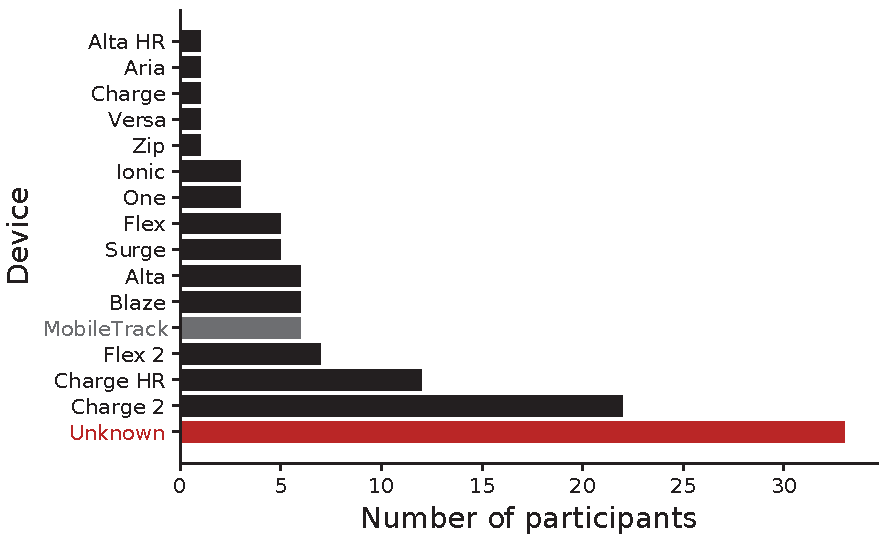
\includegraphics[width=0.6\textwidth]{figs/devices}
\caption{\textbf{Fitbit devices.}  The bars indicate the numbers of
  participants whose fitness tracking data came from each model of
  Fitbit device.  ``MobileTrack'' refers to participants who used
  smartphone accelerometer information to track their activity via the
  Fitbit smartphone app.
  ``Unknown''  denotes participants whose device information was not
  specified in their Fitbit data.}
\label{fig:devices}
\end{figure}


\begin{sidewaysfigure}[p]
\centering
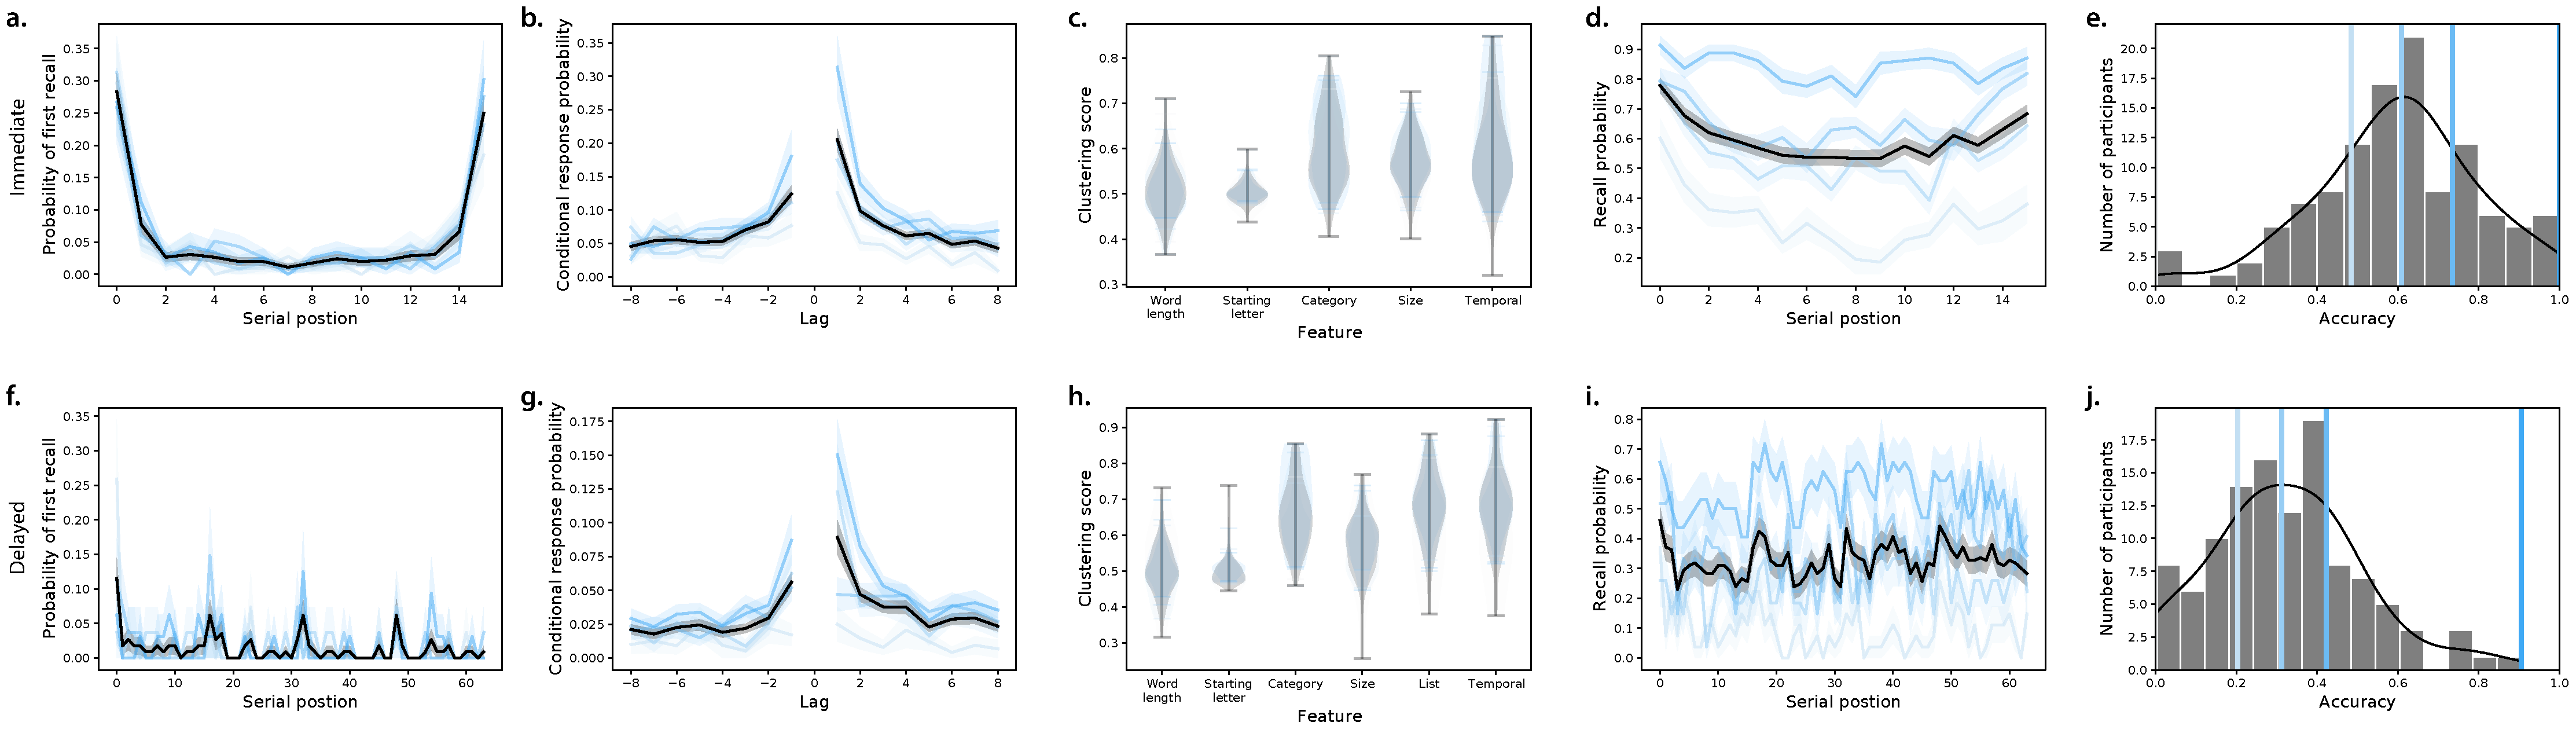
\includegraphics[width=1\textwidth]{figs/free_recall_behavior}
\caption{\textbf{Free recall behavioral results.  a--e. Immediate free
  recall.}  \textbf{a. Probability of first recall.}  Probability of
recalling each studied word first, as a function of its presentation
position.  \textbf{b. Lag Conditional Response Probability.}
Probability of recalling the word presented at position $i +
\mathrm{Lag}$ following the recall of the word presented at position
$i$.  \textbf{c. Clustering scores.}  Each score denotes participants'
tendencies to successively recall (cluster) words according to the
given feature dimension~\citep{PolyEtal09}: word length, starting letter, (semantic)
category, size (large or small), or presentation position (temporal).
\textbf{d. Serial position curve.}  Probability of recalling each word
as a function of its presentation position.  \textbf{e. Recall
  accuracy.}  Distribution of the average proportions of recalled
words, across all lists studied by each participant.  \textbf{f--j.
  Delayed free recall.}  These panels are in the same formats as
Panels a -- e, but they reflect performance on the delayed free recall
memory tests.  All panels: error bars and error ribbons denote bootstrap-estimated
95\% confidence intervals.  Shading (saturation) denotes results for
different subsets of participants, according to the average
proportion of words they remembered (group boundaries are indicated
by the colored lines in Panels e and j).}
\label{fig:fr_behavioral}
\end{sidewaysfigure}

\begin{sidewaysfigure}[p]
\centering
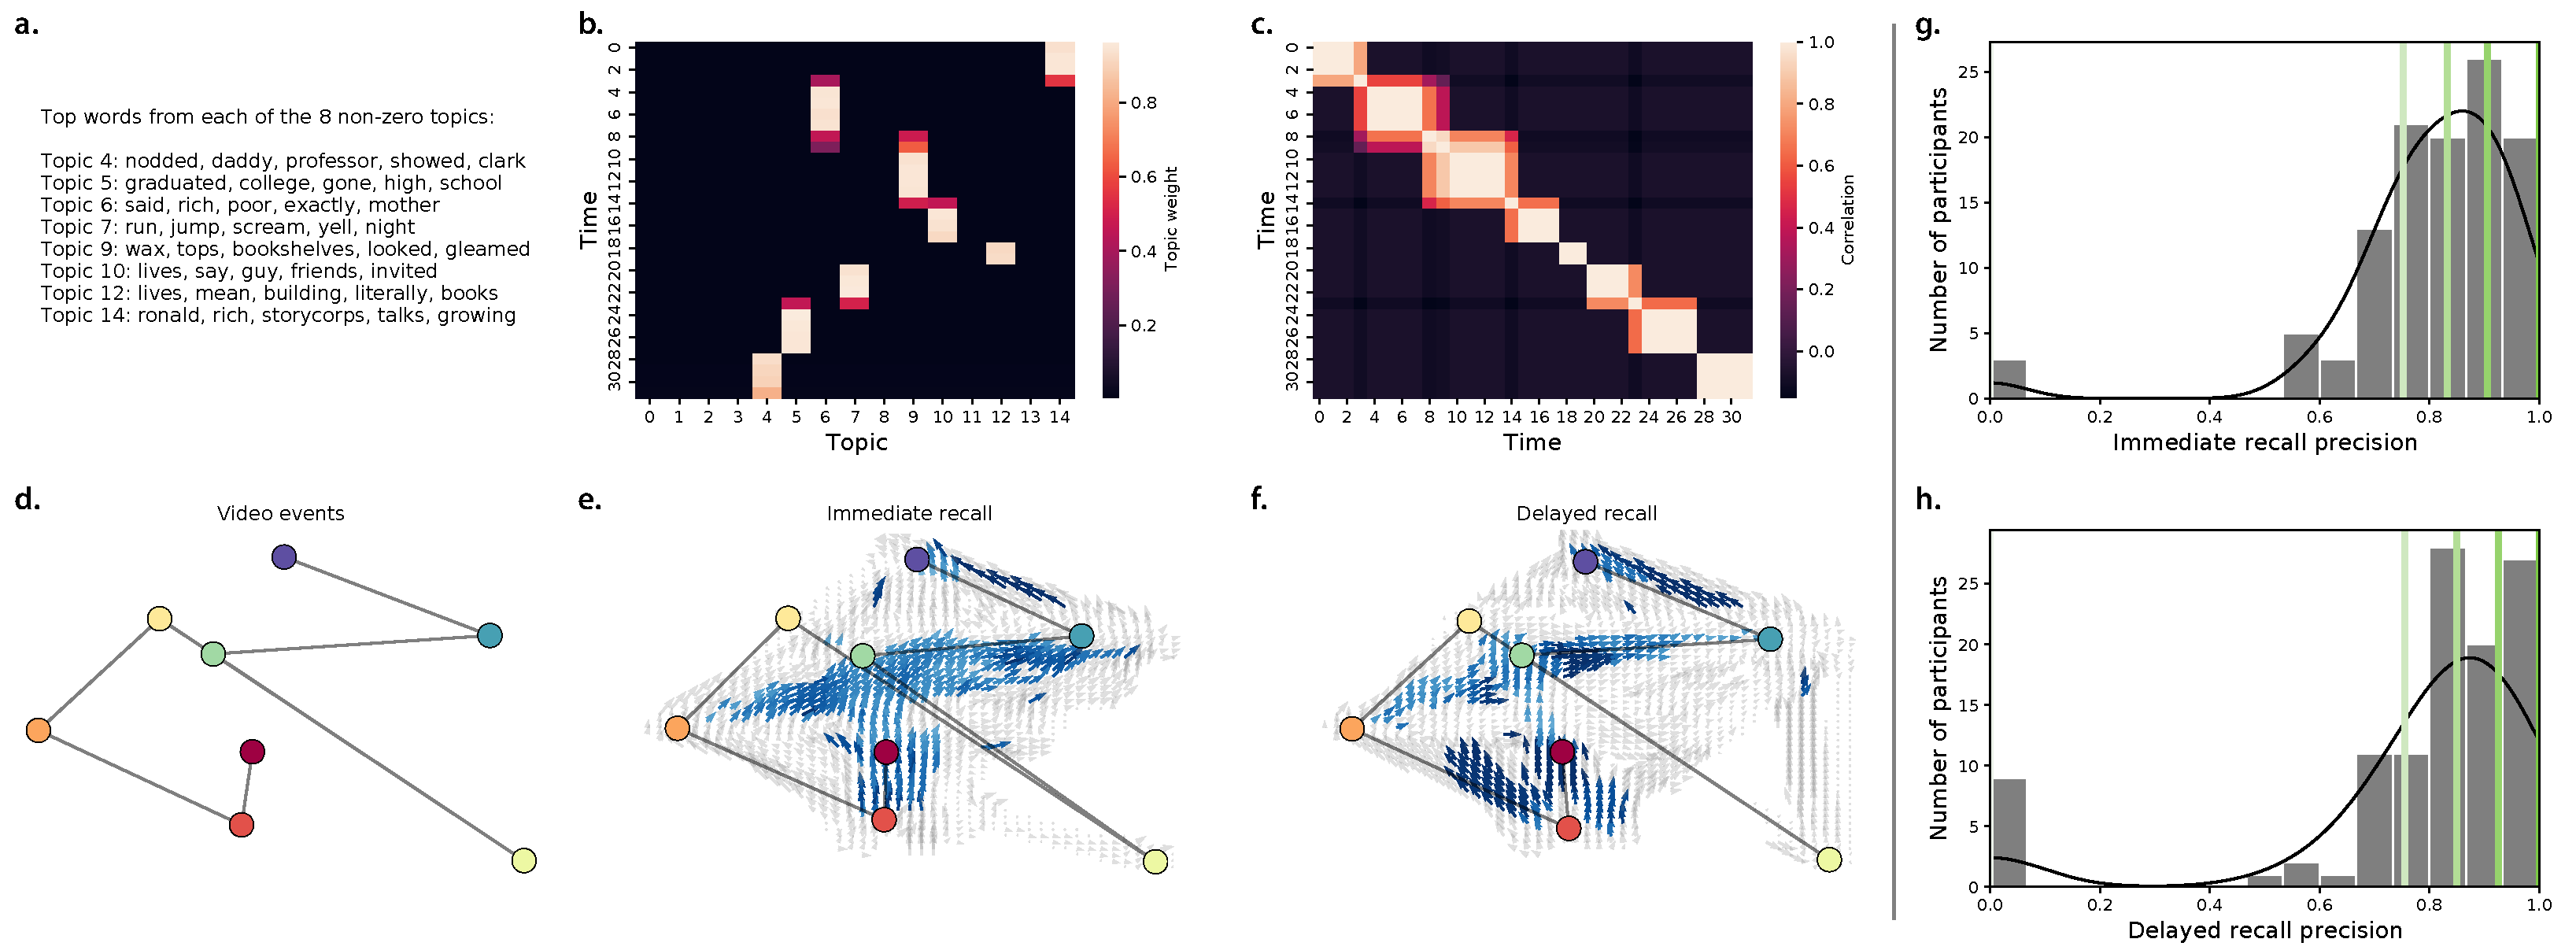
\includegraphics[width=1\textwidth]{figs/naturalistic_recall_behavior}
\caption{\textbf{Naturalistic recall behavioral results.}
  \textbf{a. Identified topics.}  Applying a topic model to a series
  of sliding windows of the video's transcript~\citep{HeusEtal21}
  revealed a set of 13 unique (non-trivial) topics.  The Panel
  displays the 5 top-weighted words from each topic.  \textbf{b. Topic
  timecourse of the video.}  Each row displays the topic weights for a
single moment of the video.  \textbf{c. Topic correlation matrix.}  The
correlations between the topic vectors for each pair of moments from
the video reveals an event-like block diagonal structure.
\textbf{d. Video topic trajectory.}  The topic video's topic
timecourse (Panel b) has been projected onto 2-dimensions using
Uniform Manifold Approximation and
Projection~\citep[UMAP;][]{McInEtal18}.  Each colored dot reflects an
event, identified by applying a Hidden Markov Model to the video's
topic timecourse~\citep{BaldEtal17, HeusEtal21}.  Red dots denote
earlier timepoints in the video and blue dots denote later
timepoints.  \textbf{e. Immediate recall trajectory.}  The black curve
displays the average
topic timecourse (projected into 2D using UMAP), obtained by applying the topic model shown in Panel A
to the participants' written transcripts from the immediate recall
test.  The arrows denote agreement across participants in the
directions of their topic trajectories, for participants whose
trajectories intersected the corresponding region of topic space.
Blue arrows denote reliable agreement across participants ($p < 0.05$, corrected).
\textbf{f. Delayed recall trajectory.} This panel is in the same
format as Panel e, but displays the trajectory for participants'
delayed recall of the video.  \textbf{g. Immediate recall precision.}  Distribution of
average recall \textit{precision}, across all of the events each
participant recalled during the immediate recall test.  Precision is
defined as the correlation between the topic vector for a given
recalled event and the best-matching (most highly correlated) video
event's topic
vector~\citep{HeusEtal21}.  \textbf{h. Delayed recall precision.}
This panel is in the same format as Panel g, but displays the average
precision values for the delayed memory test.}
\label{fig:nat_behavioral}
\end{sidewaysfigure}

\begin{figure}[p]
\centering
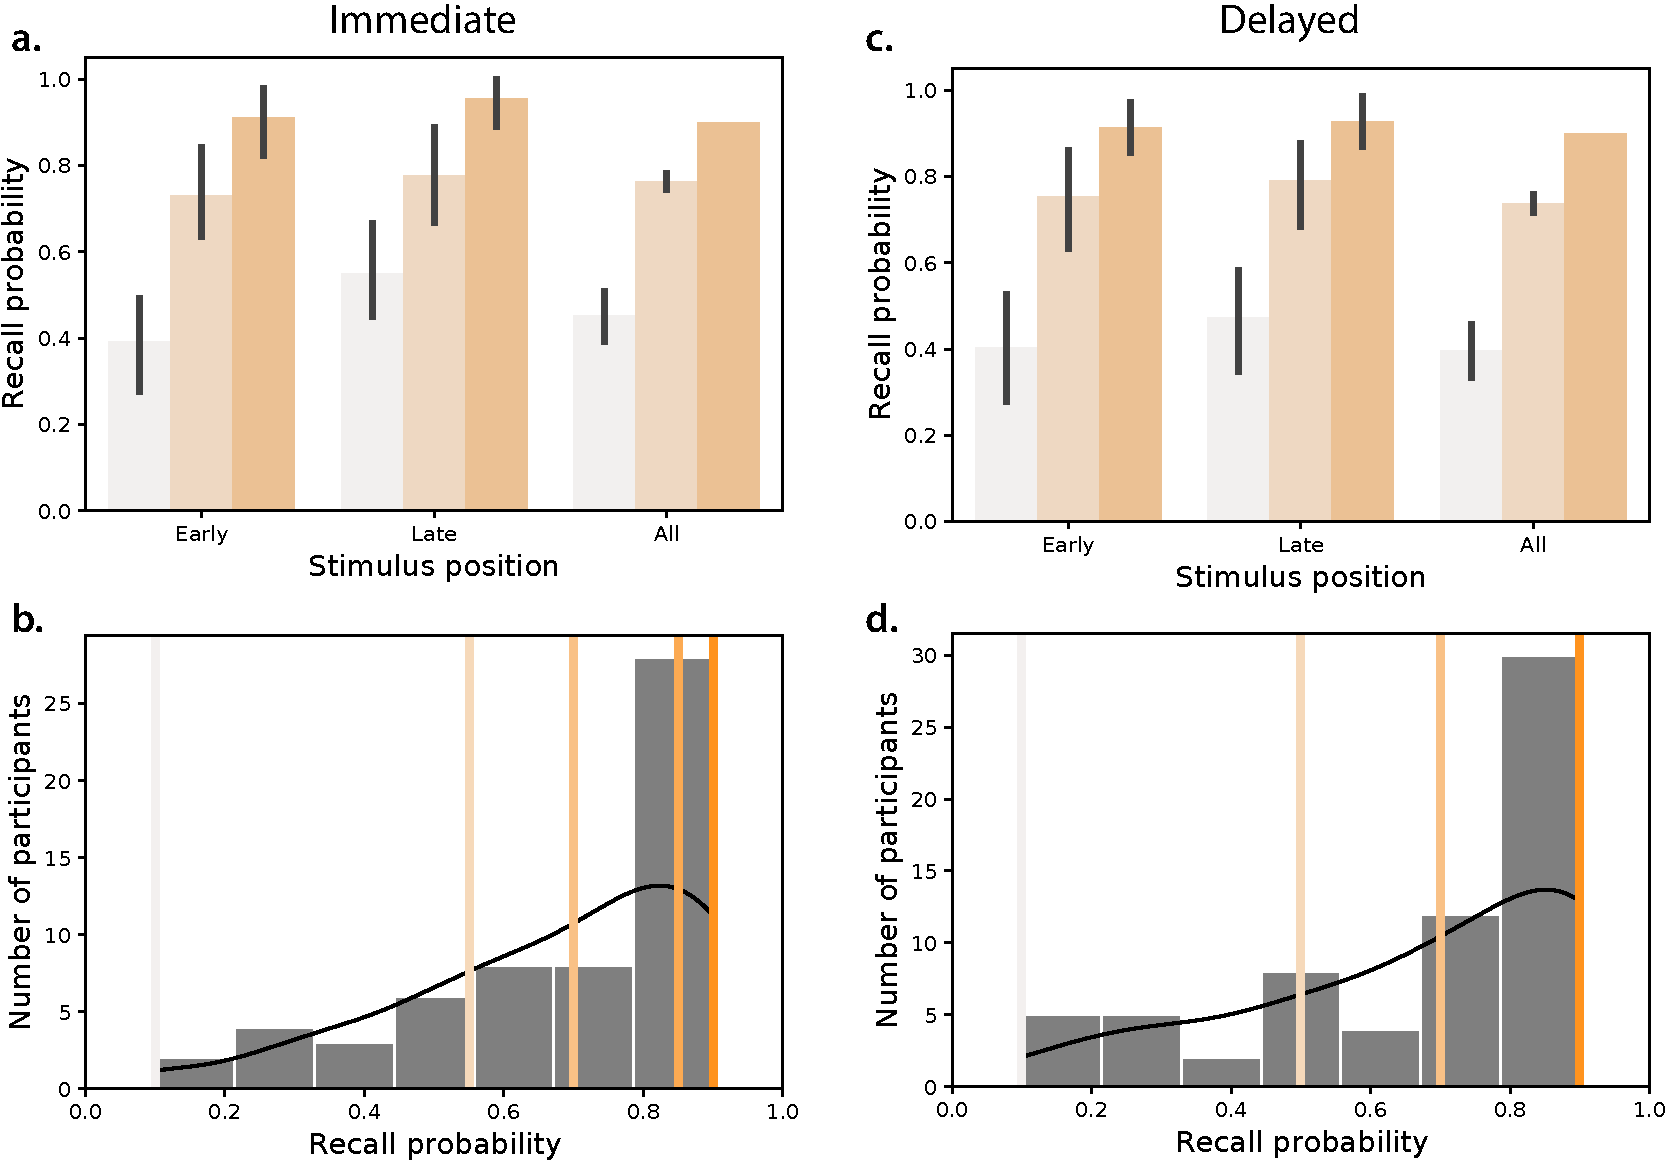
\includegraphics[width=0.6\textwidth]{figs/vocab_learning_behavior}
\caption{\textbf{Foreign language vocabulary learning behavioral
    results.}  \textbf{a. Immediate recall.}  Average proportions of
  correctly identified Gaelic-English word pairs from \textit{early} (first 3) and
\textit{late} (last 3) study positions, or aggregated over
\textit{all} study positions.  \textbf{b. Distribution of proportion
  of correctly recalled pairs on the immediate memory test.}  The colored
lines indicate quartile boundaries, and correspond to the coloring in
Panel a.  Note that the right-most edge of the third quartile overlaps
with the top quartile, since over 25\% of the participants correctly recalled
90\% of the word pairs correctly, but no participant achieved 100\%
accuracy.  \textbf{c--d. Delayed recall.}  These panels are in the
same formats as Panels a and b, but reflect performance on the delayed
recall test.  The error bars in Panels a and c denote
bootstrap-estimated 95\% confidence intervals.}
\label{fig:vocab_behavioral}
\end{figure}

\begin{figure}[p]
\centering
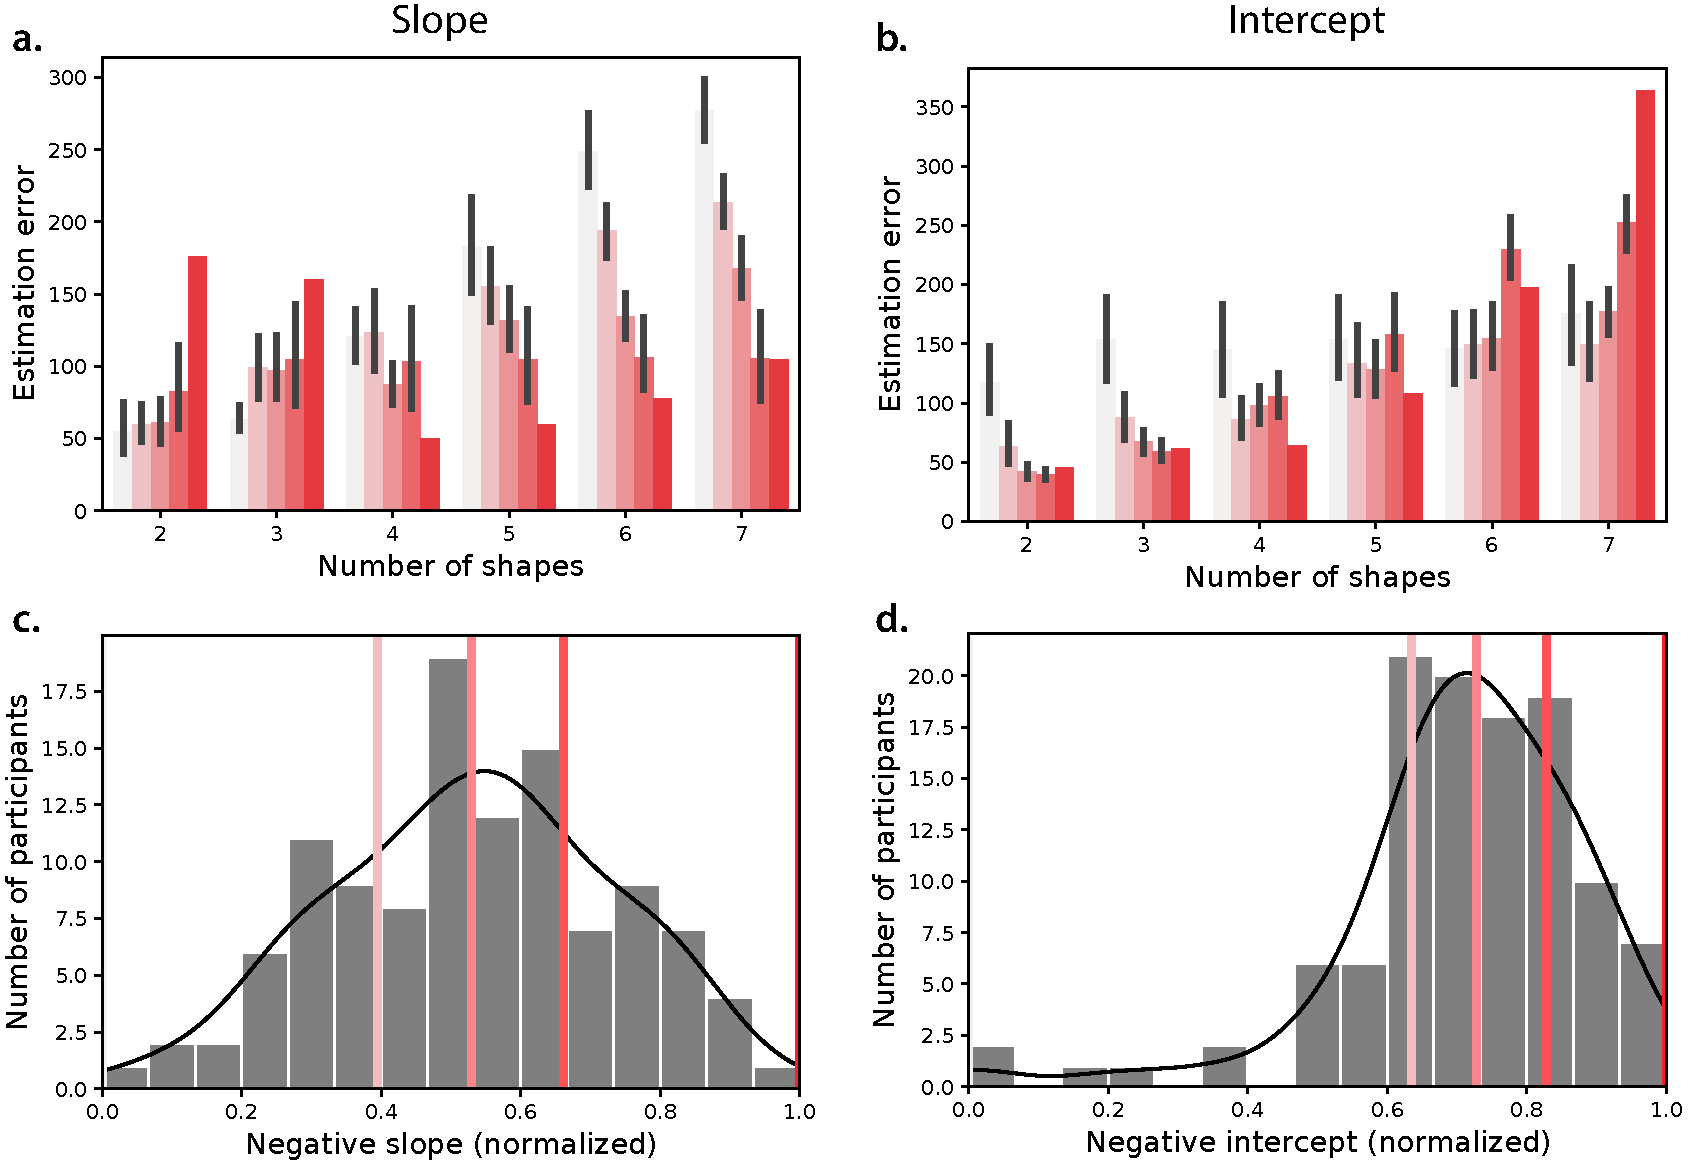
\includegraphics[width=0.6\textwidth]{figs/spatial_learning_behavior}
\caption{\textbf{Spatial learning behavioral results.}
  \textbf{a--b. Estimation error.}  Estimation
  error is defined as the Euclidean distance between each shape's
  studied and recalled positions.  The bars show the average
  estimation error (across all shapes for each memory test) versus the
  number of memorized shapes.  \textbf{a. Slope.} Estimation errors
  are broken down by the slopes of regression lines fit to each
  participant's estimation errors as a function of the number of
  memorized shapes.  Shallower slopes (i.e., smaller decreases in
  performance associated with memorizing more shapes) are reflected by
  more saturated coloring.  Error bars denote bootstrap-estimated 95\%
  confidence intervals.  \textbf{b. Intercept.}  Bars are in the same
  format as Panel a, but here estimation errors are
  broken down by the intercepts of the same regressions used in Panel
  a.  Smaller intercepts (i.e., smaller baseline errors) are reflected
  by more saturated coloring.  \textbf{c. Distribution of slopes.}
  Across-participant distribution of regression slopes.  The lines
  denote quartile boundaries (colors are matched to Panel a).  The
  slopes are multiplied by -1 and normalized to be within the [0, 1]
  interval such that (adjusted) slopes closer to 1 reflect better
  performance and slopes closer to 0 reflect worse performance.
  \textbf{b. Distribution of intercepts.}  Across-participant
  distribution of regression intercept terms.  The lines denote
  quartile boundaries (colors are matched to Panel b).  The intercepts
  are multiplied by -1 and normalized to be within the [0, 1] interval
  such that (adjusted) intercepts closer to 1 reflect better
  performance and intercepts closer to 0 reflect worse performance.}
\label{fig:spatial_behavioral}
\end{figure}

\clearpage
\begin{table}[]
\centering
\resizebox{\textwidth}{!}{%
\begin{tabular}{p{1.5in}p{4in}p{1.5in}}
\textbf{Abbreviation}   & \textbf{Description}
  & \textbf{Units}                           \\
  \hline
Resting HR              & Average daily resting heart rate                                                                                                                                                     & beats per minute (BPM)                   \\
  \hline
HR variability          & Heart rate variability (average daily variation between heartbeats)                                                                                                                  & milliseconds (ms)                        \\
  \hline
Steps                   & Number of steps taken each day                                                                                                                                                       & steps (count)                            \\
  \hline
Distance                & Estimated distance traveled each day                                                                                                                                                 & kilometers (km)                          \\
  \hline
Elevation               & Estimated daily elevation gain                                                                                                                                                       & feet (ft)                                \\
  \hline
Floors climbed          & Estimated number of daily floors climbed                                                                                                                                             & floors (count)                           \\
  \hline
Light activity          & Number of estimated daily minutes spent doing low-intensity activity                                                                                                                 & minutes (min)                            \\
  \hline
Fair activity           & Number of estimated daily minutes spent doing moderate-intensity activity                                                                                                            & minutes (min)                            \\
  \hline
High intensity activity & Number of estimated daily minutes spent doing high-intensity activity                                                                                                                & minutes (min)                            \\
  \hline
Excess calories         & Number of estimated daily calories burned minus estimated calorie intake                                                                                                             & calories (cal)                           \\
  \hline
Out-of-range HR, OOR mins         & Number of daily minutes spent with a heart rate lower than the "fat burn" heart rate zone (50\% of the maximum heart rate); maximum heart rate is defined as 220 minus age, in years & minutes (min)                            \\
  \hline
Fat burn HR             & Number of daily minutes spent with a heart rate between 50\% and 69\% of the maximum heart rate                                                                                      & minutes (min)                            \\
  \hline
Cardio HR               & Number of daily minutes spent with a heart rate between 70\% and 84\% of the maximum heart rate                                                                                      & minutes (min)                            \\
  \hline
Peak HR                 & Number of daily minutes spent with a heart rate between 85\% and 100\% of the maximum heart rate                                                                                     & minutes (min)                            \\
  \hline
Sleep duration          & Estimated number of hours slept during the prior 24 hour period                                                                                                                      & hours (hr)                               \\
  \hline
BMI                     & Body mass index, calculated as the
                          individual's weight (in kg) divided by their
                          height (in m) squared
  & kilograms per meter squared (kg/m\textsuperscript{2}) \\
  \hline
Body fat                & Estimated percentage of body fat (as a proportion of the individual's total weight)                                                                                                  & percentage (\%)                          \\
  \hline
Weight                  & Logged or measured weight                                                                                                                                                            & kilograms (kg)                           \\
  \hline
Water intake            & Self-reported water intake                                                                                                                                                           & 8 ounce cups (count)                     \\
  \hline
Coffee intake           & Self-reported coffee intake                                                                                                                                                          & 8 ounce cups (count)                    
\end{tabular}%
}
\caption{\textbf{Abbreviations of fitness-related measures.}  The
  abbreviations and descriptions provided in the table apply to the
  main text and supplement.}
\label{tab:abbreviations}
\end{table}

\begin{sidewaysfigure}[p]
\centering
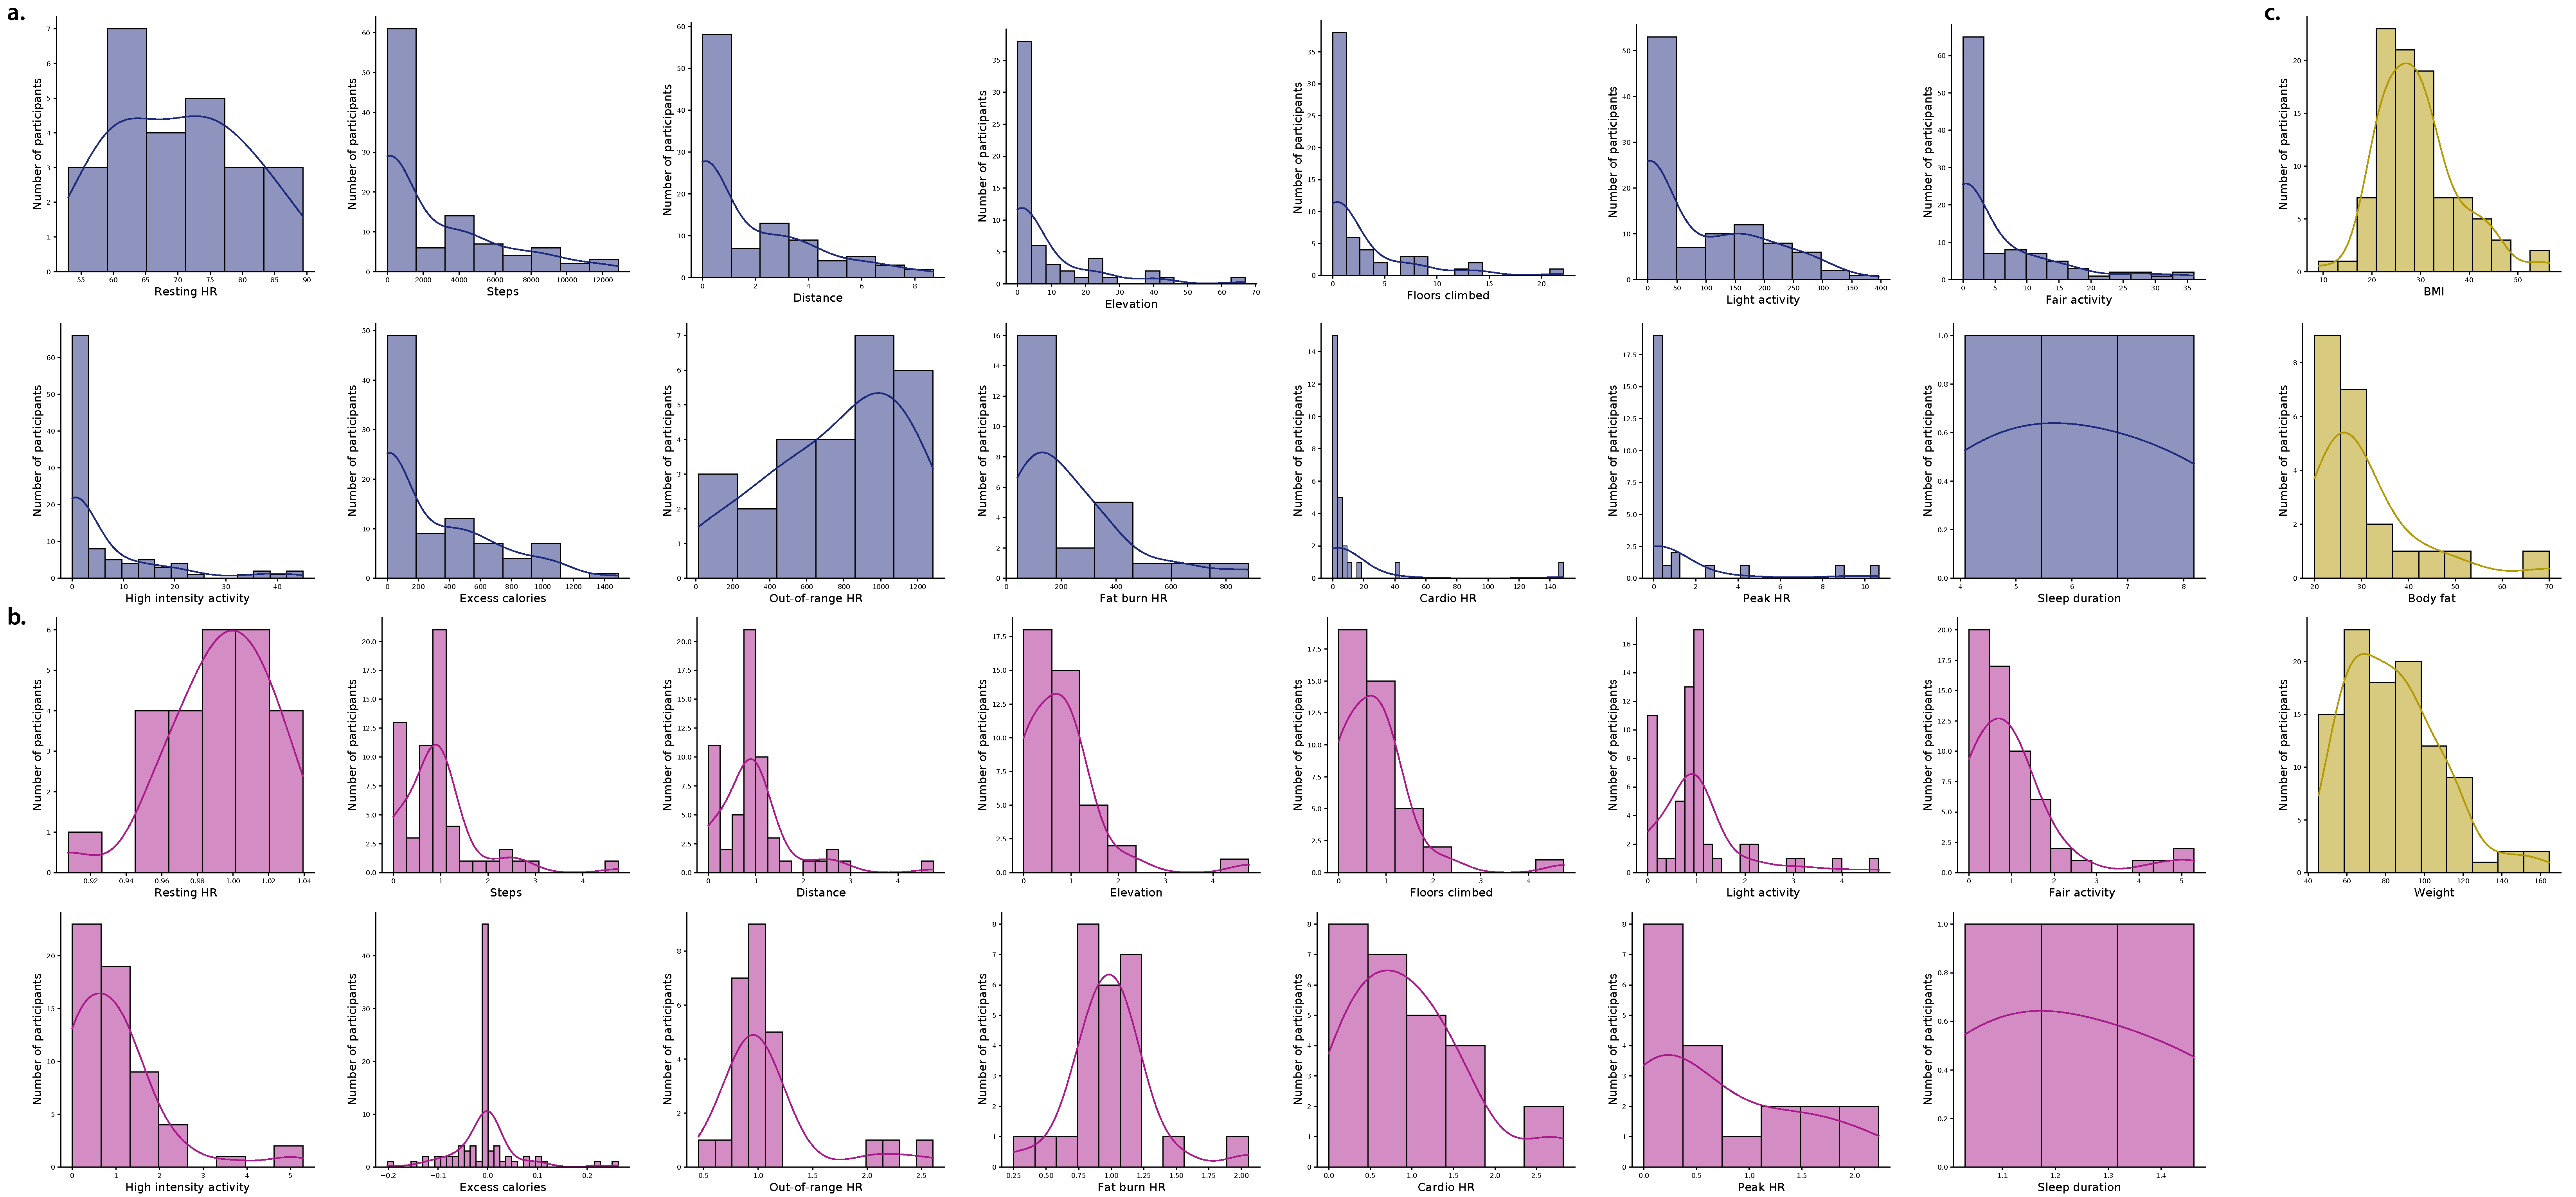
\includegraphics[width=\textwidth]{figs/fitness_distributions}
\caption{\textbf{Distributions of fitness measures.}  All
  abbreviations and measures are described in
  Table~\ref{tab:abbreviations}.  \textbf{a. Recent measures.}
  Daily values of each measure, averaged over the week prior to each
  participant's test day.  \textbf{b. Baselined measures.}  Daily
  values of each measure, averaged over the week prior to each
  participant's test day and divided by the average taken over the
  preceding 30 days.  \textbf{c. Static measures.} For each measure,
  only the most recently logged values are considered.  All panels:
  note that not all measures were captured for all participants.  Only
participants whose Fitbit records logged each given measure are
included in the distribution(s) for that measure.}
\label{fig:fitness_dists}
\end{sidewaysfigure}

\begin{sidewaysfigure}[p]
\centering
\includegraphics[width=\textwidth]{figs/fitness_dists_immediate}
\caption{\textbf{Distributions of fitness measures, broken down
    by immediate task performance.}  The distributions of recent
  (Panel a), baselined (Panel b), and static (Panel c) fitness
  measures (Tab.~\ref{tab:abbreviations}) are broken down by
  participants' performance on each immediate recall test
  (Figs.~\immediateBehavior, \ref{fig:fr_behavioral},
  \ref{fig:nat_behavioral}, \ref{fig:vocab_behavioral}, and \ref{fig:spatial_behavioral})}
\label{fig:fitness_dists_immediate}
\end{sidewaysfigure}

\begin{sidewaysfigure}[p]
\centering
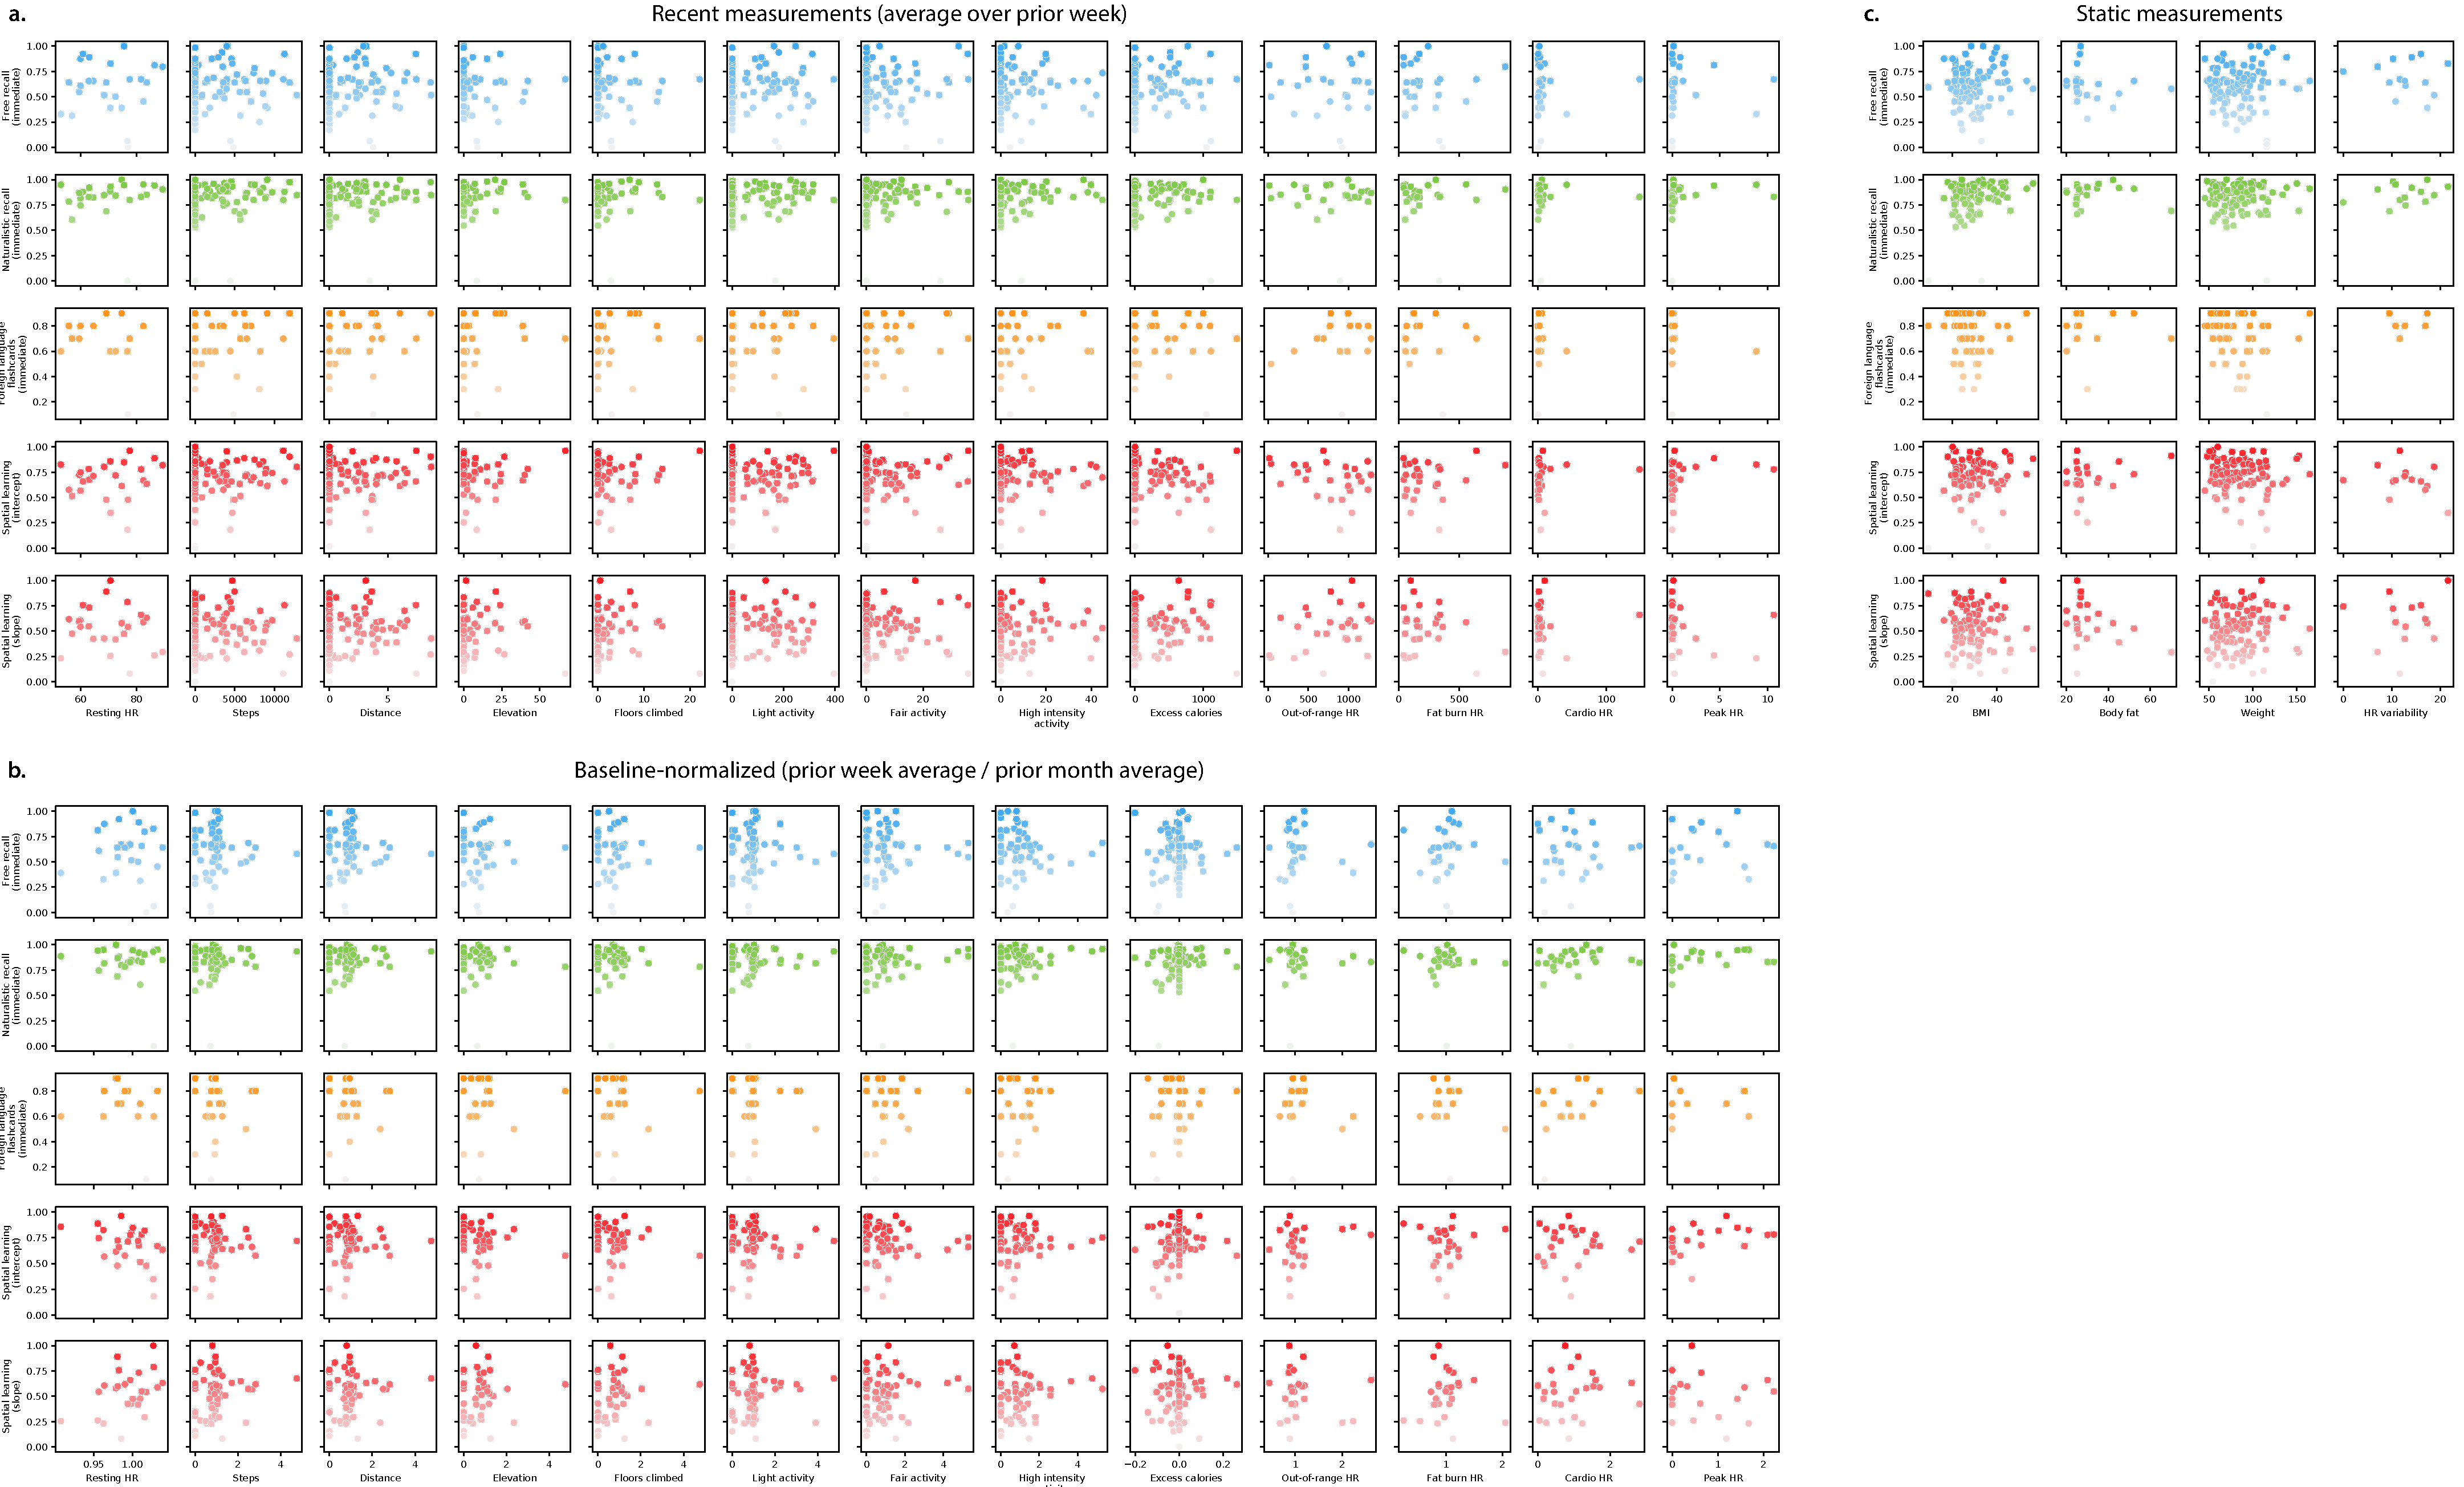
\includegraphics[width=\textwidth]{figs/fitness_scatter_immediate}
\caption{\textbf{Scatterplots of fitness measures versus
    immediate task performance measures.}  The scatterplots of recent
  (Panel a), baselined (Panel b), and static (Panel c) fitness
  measures (Tab.~\ref{tab:abbreviations}) are plotted against 
  participants' performance on each immediate recall test
  (Figs.~\immediateBehavior, \ref{fig:fr_behavioral}, \ref{fig:nat_behavioral}, \ref{fig:vocab_behavioral}, and \ref{fig:spatial_behavioral})}
\label{fig:fitness_scatters_immediate}
\end{sidewaysfigure}

\begin{sidewaysfigure}[p]
\centering
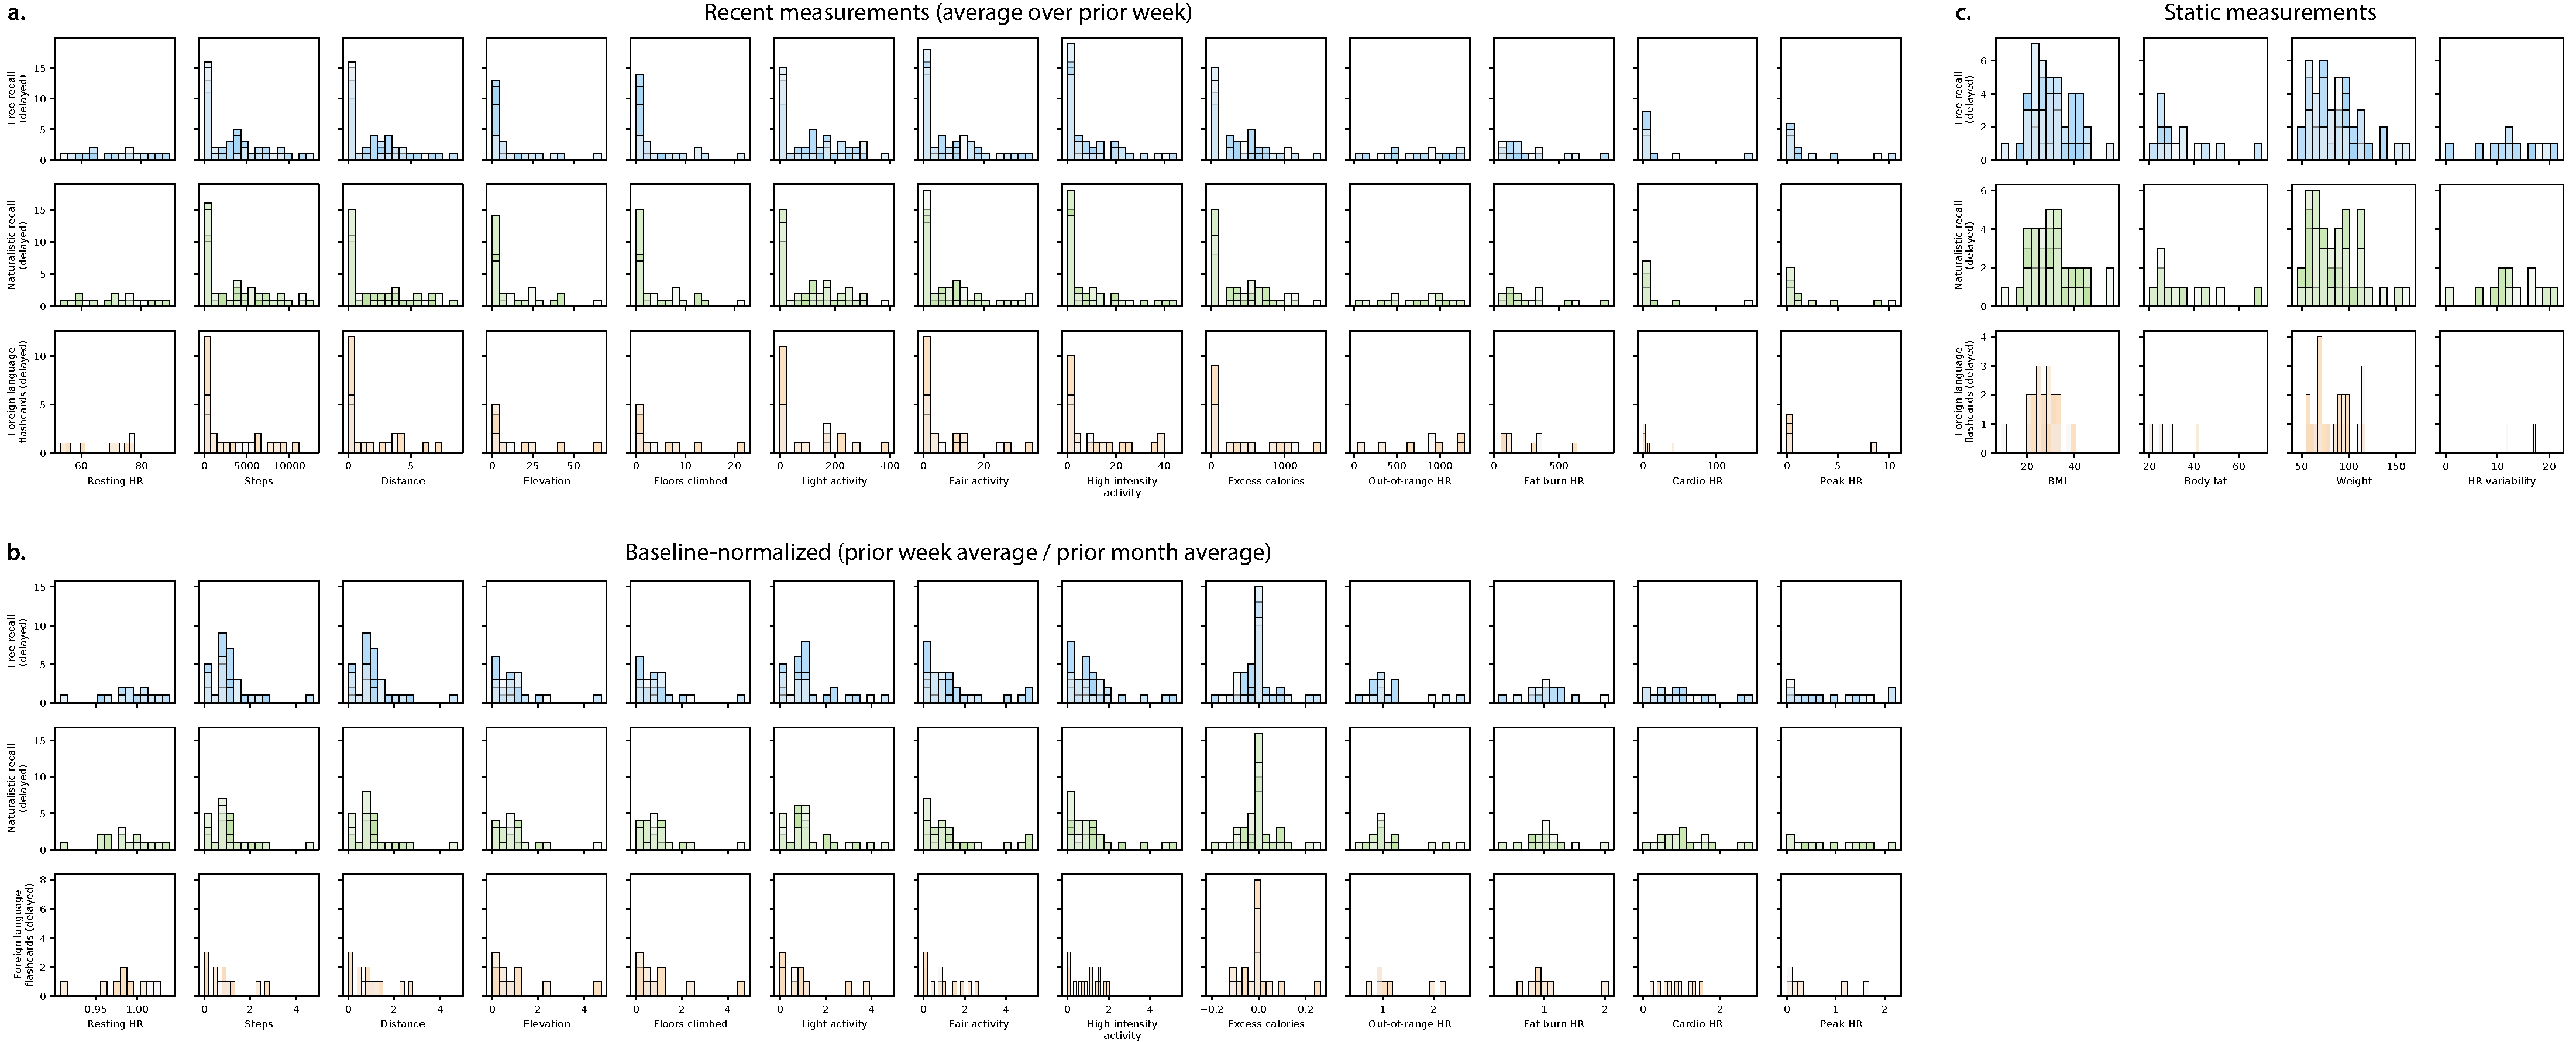
\includegraphics[width=\textwidth]{figs/fitness_dists_delayed}
\caption{\textbf{Distributions of fitness measures, broken down
    by delayed task performance.} The distributions of recent
  (Panel a), baselined (Panel b), and static (Panel c) fitness
  measures (Tab.~\ref{tab:abbreviations}) are broken down by
  participants' performance on each delayed recall test
  (Figs.~\delayedBehavior, \ref{fig:fr_behavioral},
  \ref{fig:nat_behavioral}, and \ref{fig:vocab_behavioral})}
\label{fig:fitness_dists_delayed}
\end{sidewaysfigure}

\begin{sidewaysfigure}[p]
\centering
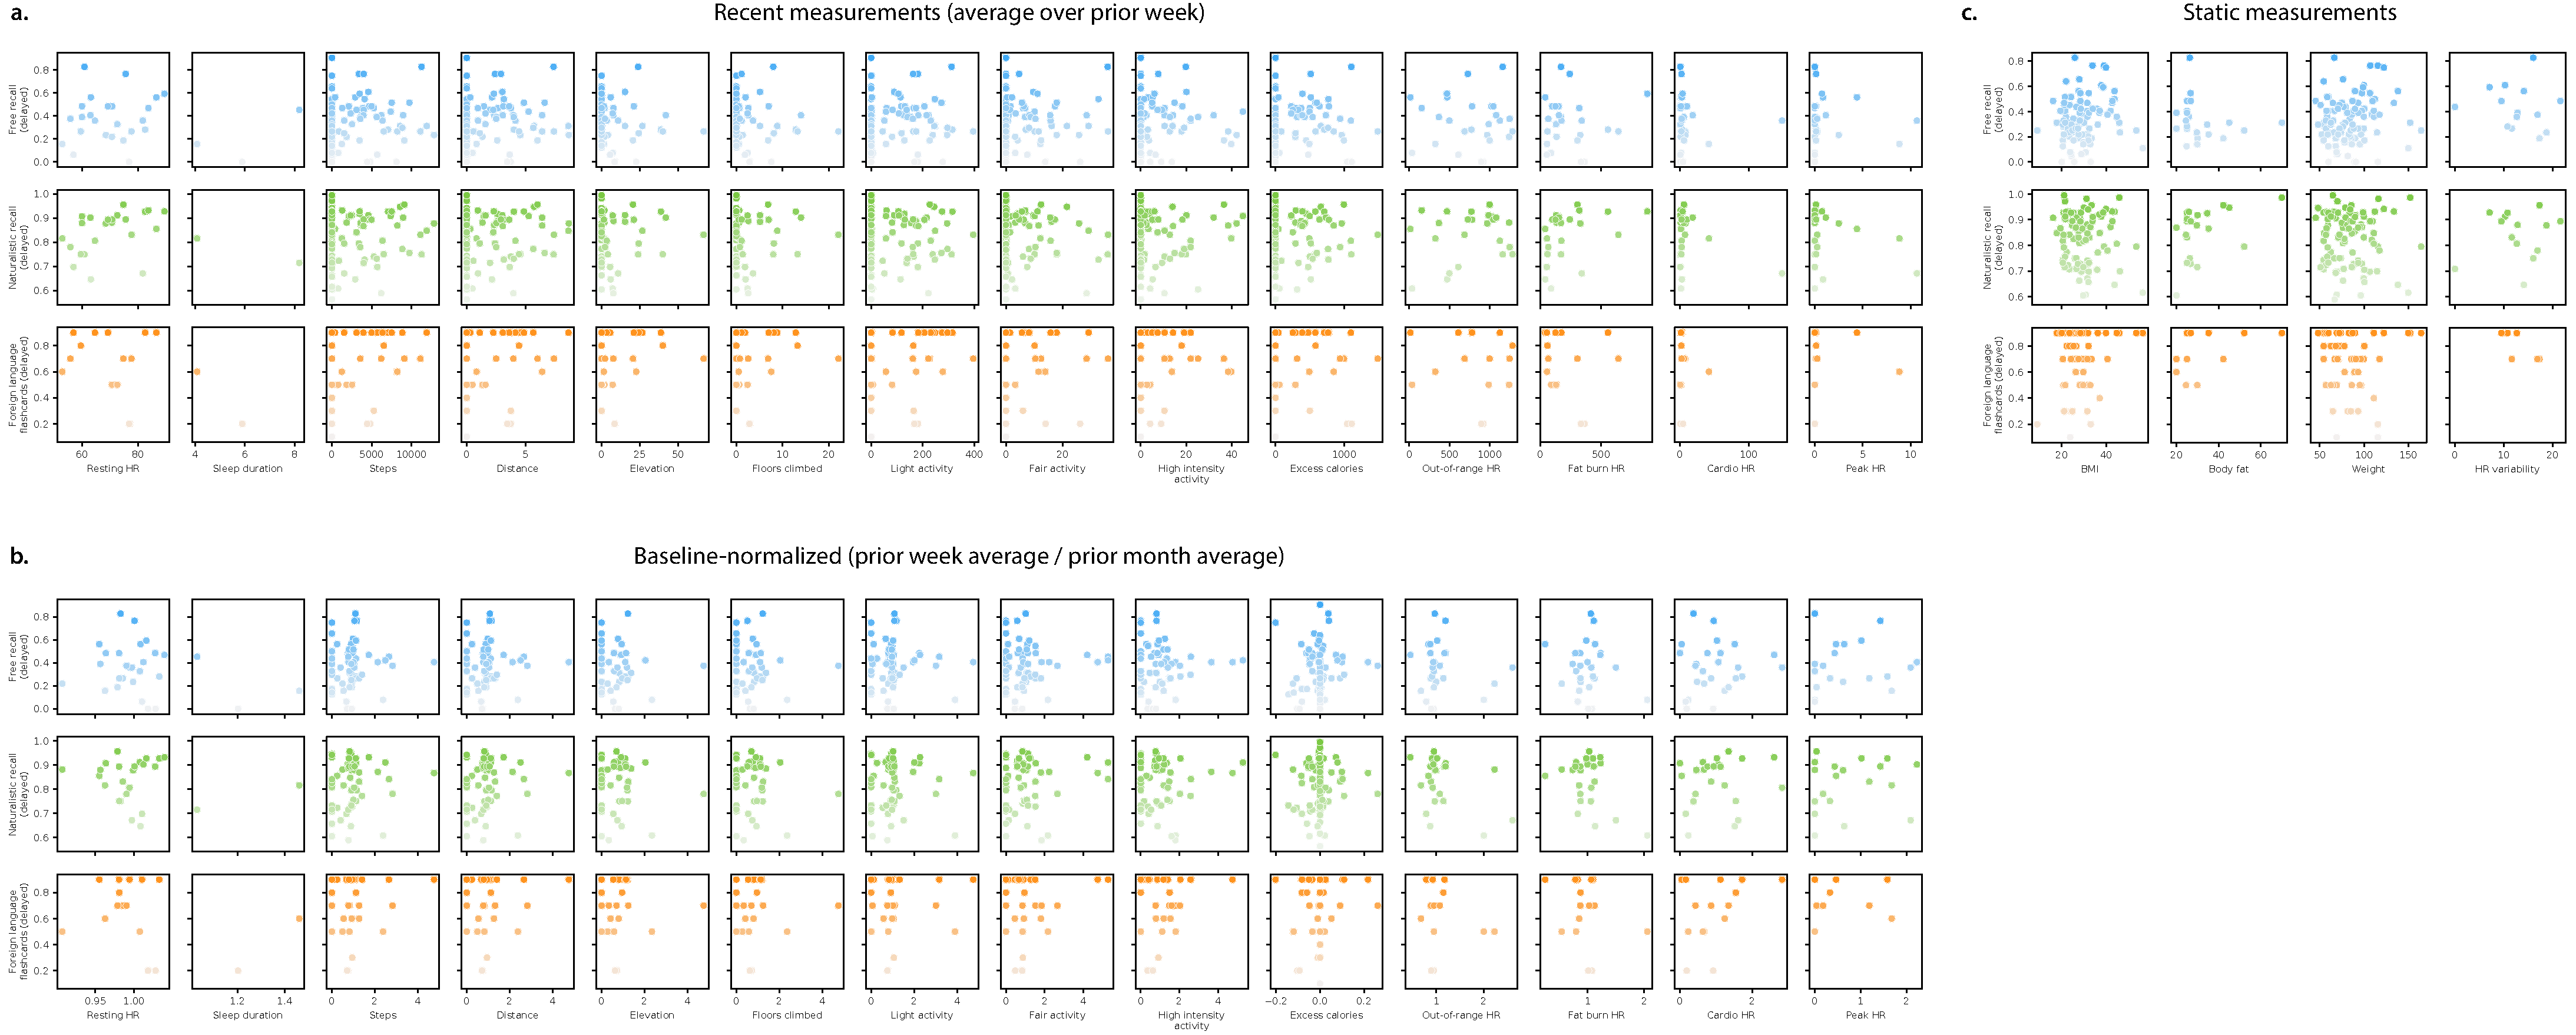
\includegraphics[width=\textwidth]{figs/fitness_scatter_delayed}
\caption{\textbf{Scatterplots of fitness measures versus
    delayed task performance measures.} The scatterplots of recent
  (Panel a), baselined (Panel b), and static (Panel c) fitness
  measures (Tab.~\ref{tab:abbreviations}) are plotted against 
  participants' performance on each delayed recall test
  (Figs.~\delayedBehavior, \ref{fig:fr_behavioral},
  \ref{fig:nat_behavioral}, and \ref{fig:vocab_behavioral})}
\label{fig:fitness_scatters_delayed}
\end{sidewaysfigure}

\begin{figure}[p]
\centering
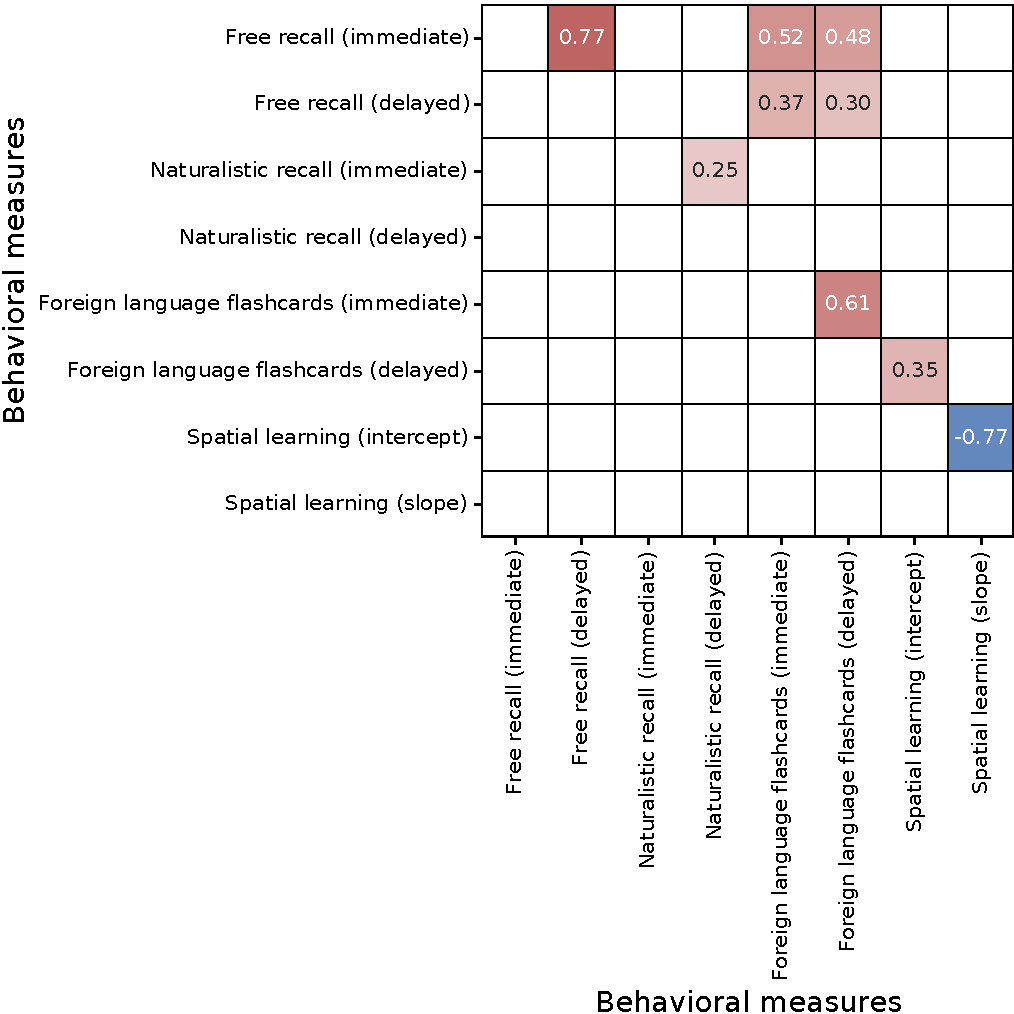
\includegraphics[width=0.4\textwidth]{figs/behavior_behavior_correlations}
\caption{\textbf{Bootstrap-estimated reliable correlations between
    behavioral measures.}  The measures are described and summarized in the
  distributions shown in Figures~\ref{fig:fr_behavioral},
  \ref{fig:nat_behavioral}, \ref{fig:vocab_behavioral}, and
  \ref{fig:spatial_behavioral}.
The reported values denote the correlation coefficient between the
given row and column.  Only statistically reliable correlations are
displayed ($p < 0.05$, corrected; see \textit{Exploratory correlation
  analysis}, main text).}
\label{fig:behavioral_corrs}
\end{figure}

\begin{figure}[p]
\centering
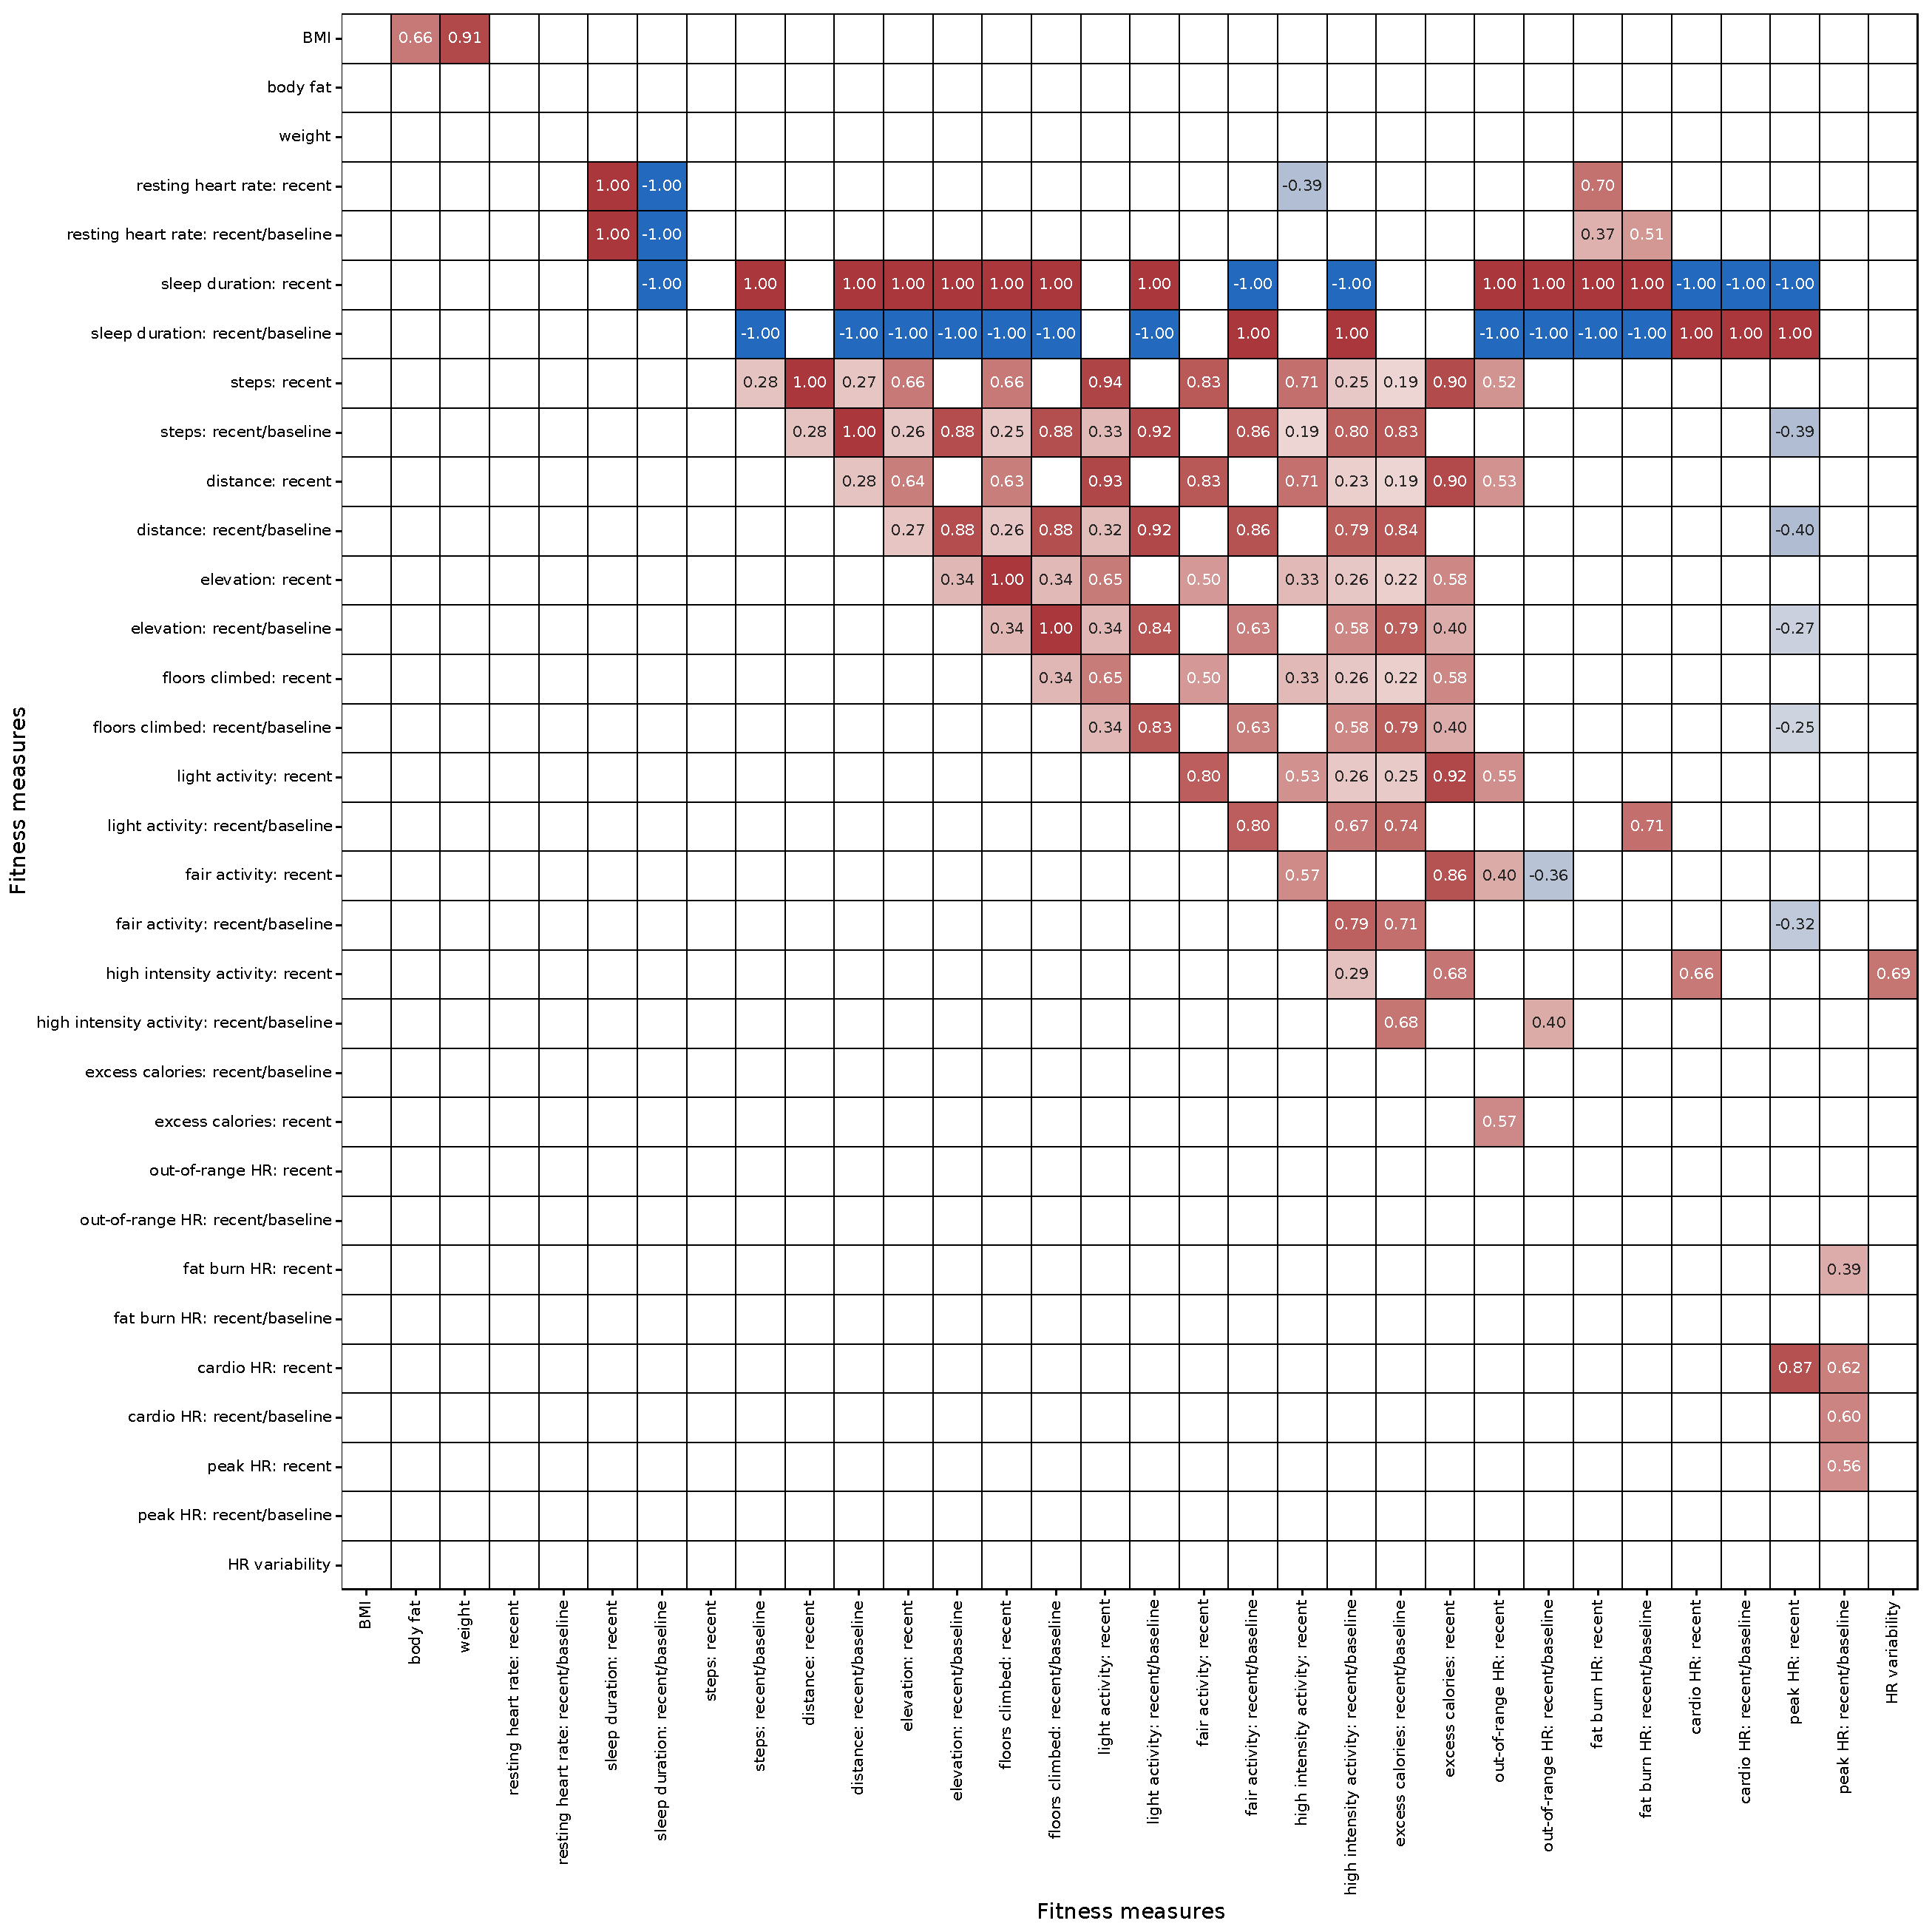
\includegraphics[width=\textwidth]{figs/fitness_fitness_correlations}
\caption{\textbf{Bootstrap-estimated reliable correlations between
    fitness measures.}  Fitness measures are described in summarized
  in Table~\ref{tab:abbreviations}.  The reported values denote the correlation coefficient between the
given row and column.  Only statistically reliable correlations are
displayed ($p < 0.05$, corrected; see \textit{Exploratory correlation
  analysis}, main text).}
\label{fig:fitness_corrs}
\end{figure}

\begin{figure}[p]
\centering
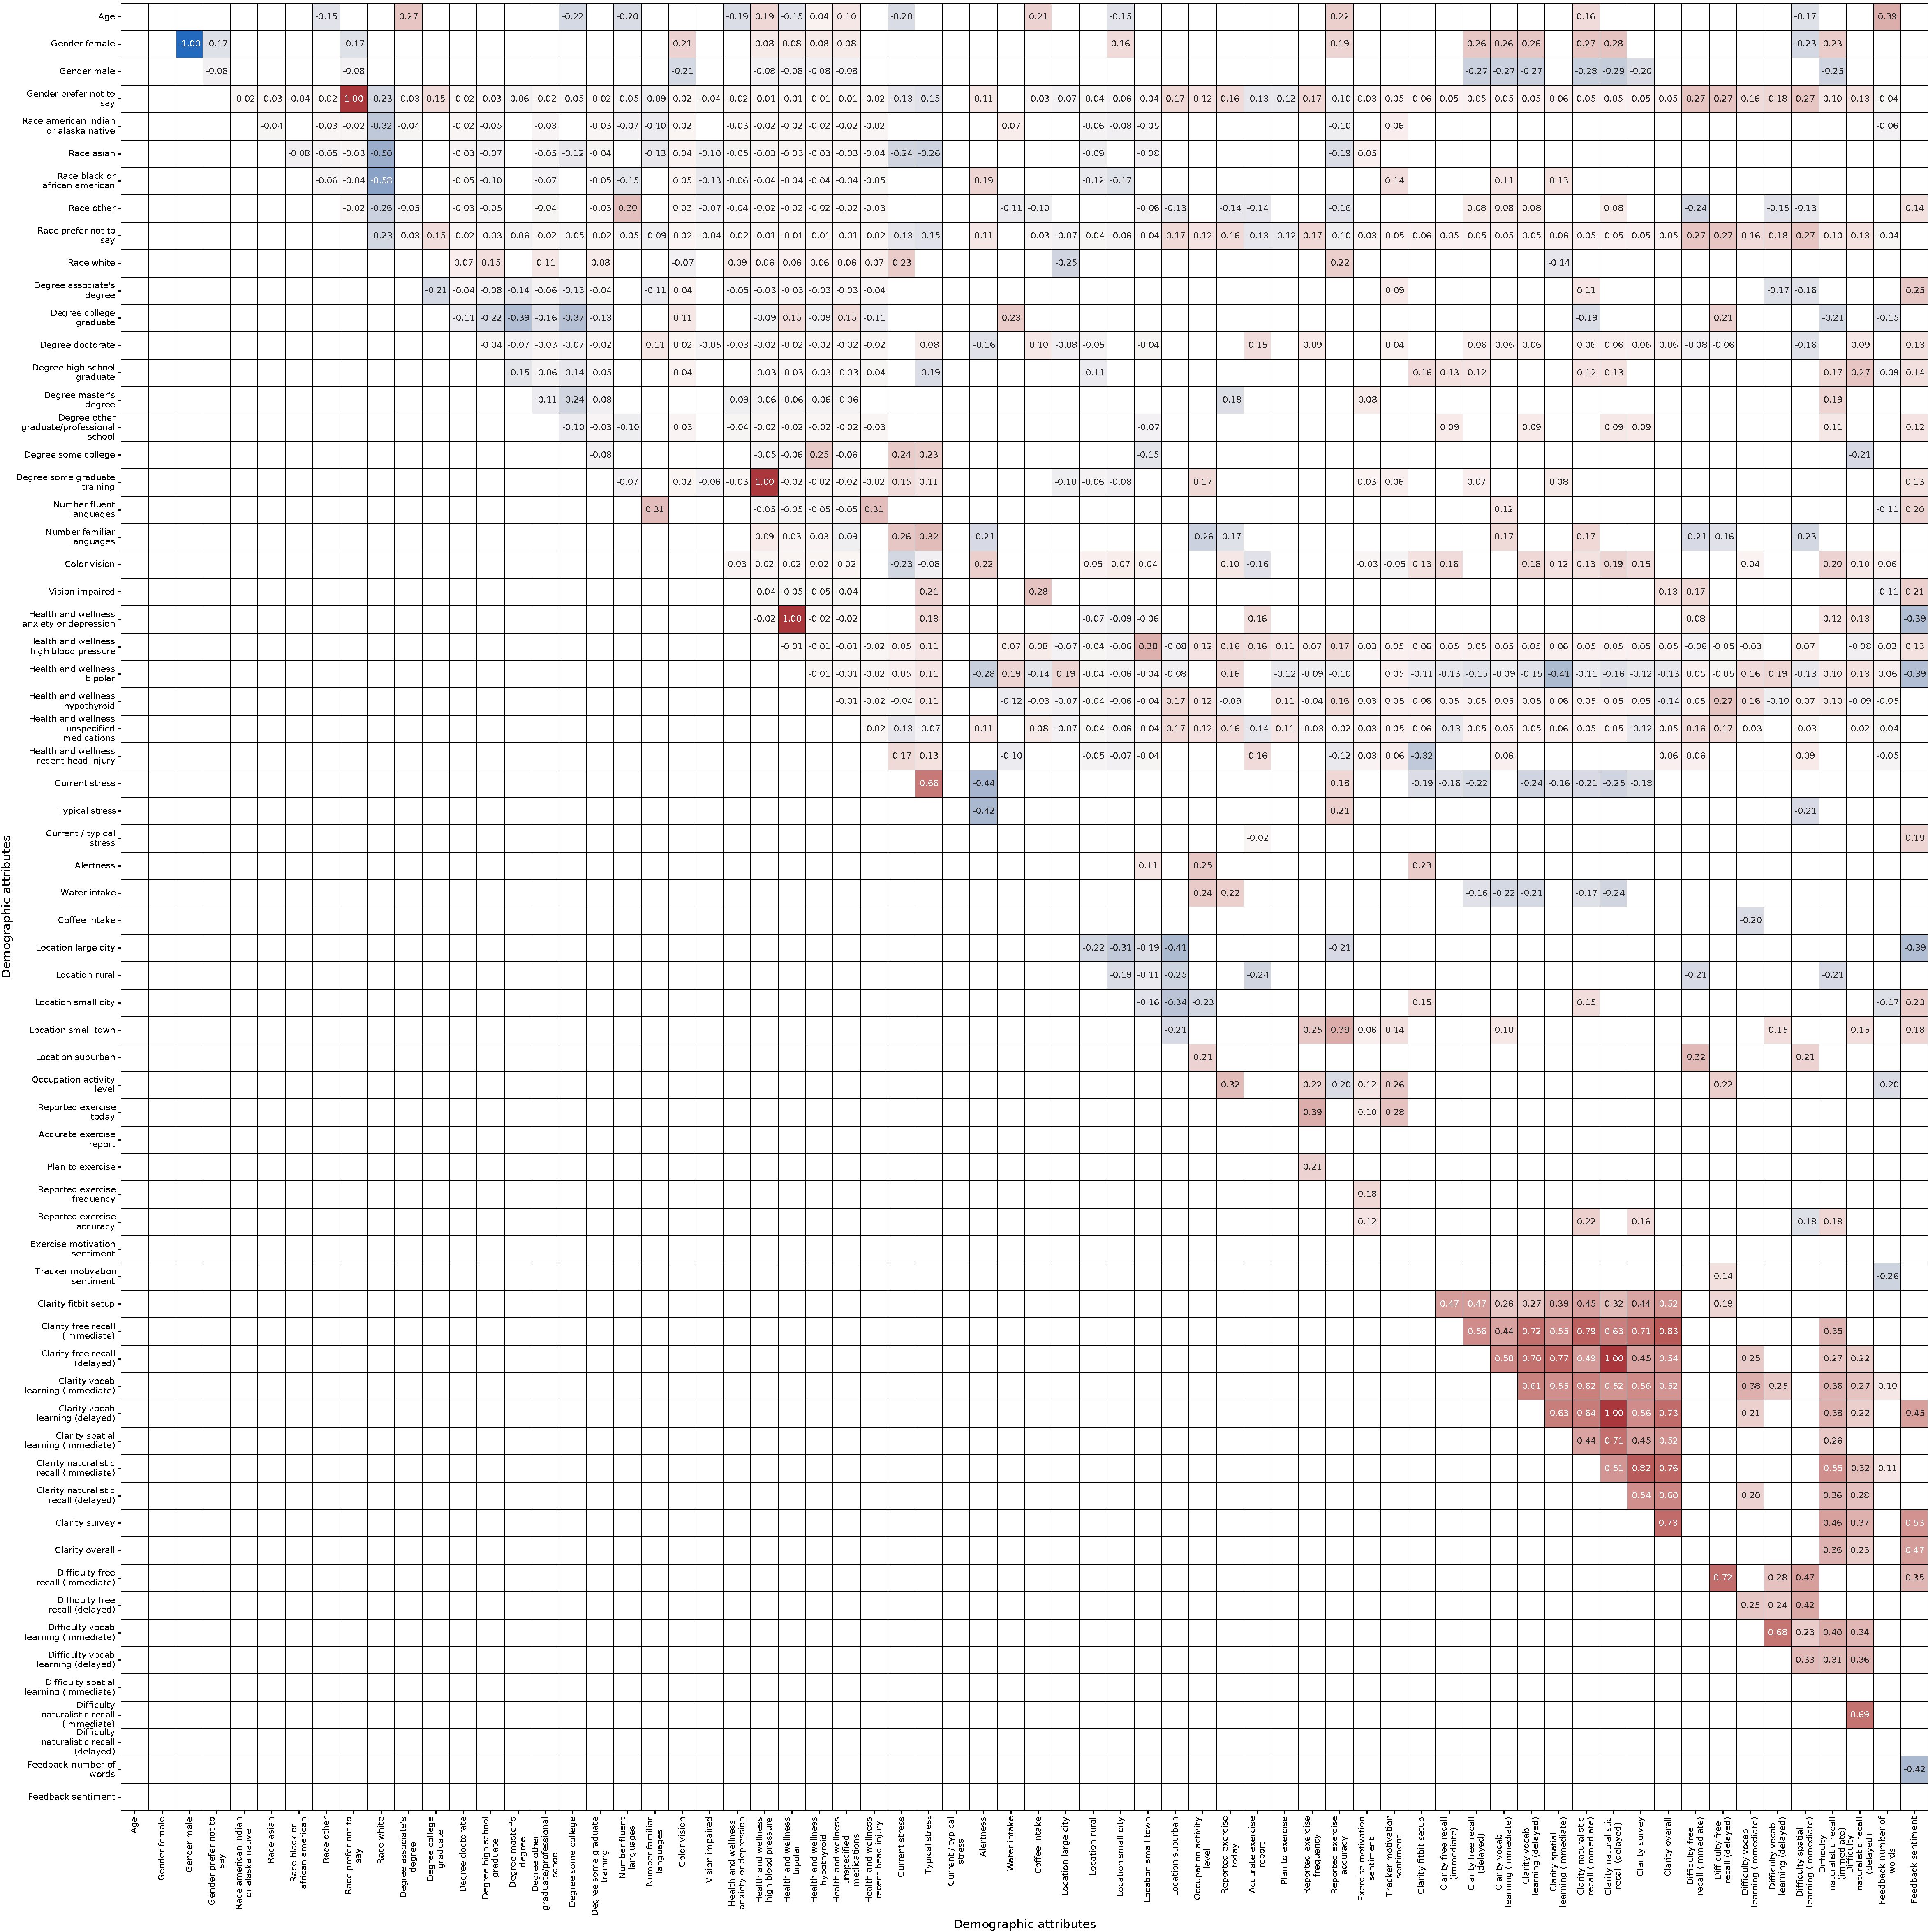
\includegraphics[width=\textwidth]{figs/survey_survey_correlations}
\caption{\textbf{Bootstrap-estimated reliable correlations between
    demographic measures.}  Demographic measures are described in the
  main text (\textit{Participants}).  The reported values denote the correlation coefficient between the
given row and column.  Only statistically reliable correlations are
displayed ($p < 0.05$, corrected; see \textit{Exploratory correlation
  analysis}, main text).}
\label{fig:survey_corrs}
\end{figure}

\begin{sidewaysfigure}[p]
\centering
\includegraphics[width=\textwidth]{figs/behavior_fitness+survey_correlations}
\caption{\textbf{Bootstrap-estimated reliable correlations between
    behavioral measures and fitness or demographic measures.}  All
  measures and abbreviations in this figure use the same notations as
  Figures~\ref{fig:behavioral_corrs}, \ref{fig:fitness_corrs}, and
  \ref{fig:survey_corrs}.  Only statistically reliable correlations are
displayed ($p < 0.05$, corrected; see \textit{Exploratory correlation
  analysis}, main text).}
\label{fig:fitness_survey_corrs}
\end{sidewaysfigure}

\begin{figure}[p]
  \centering
  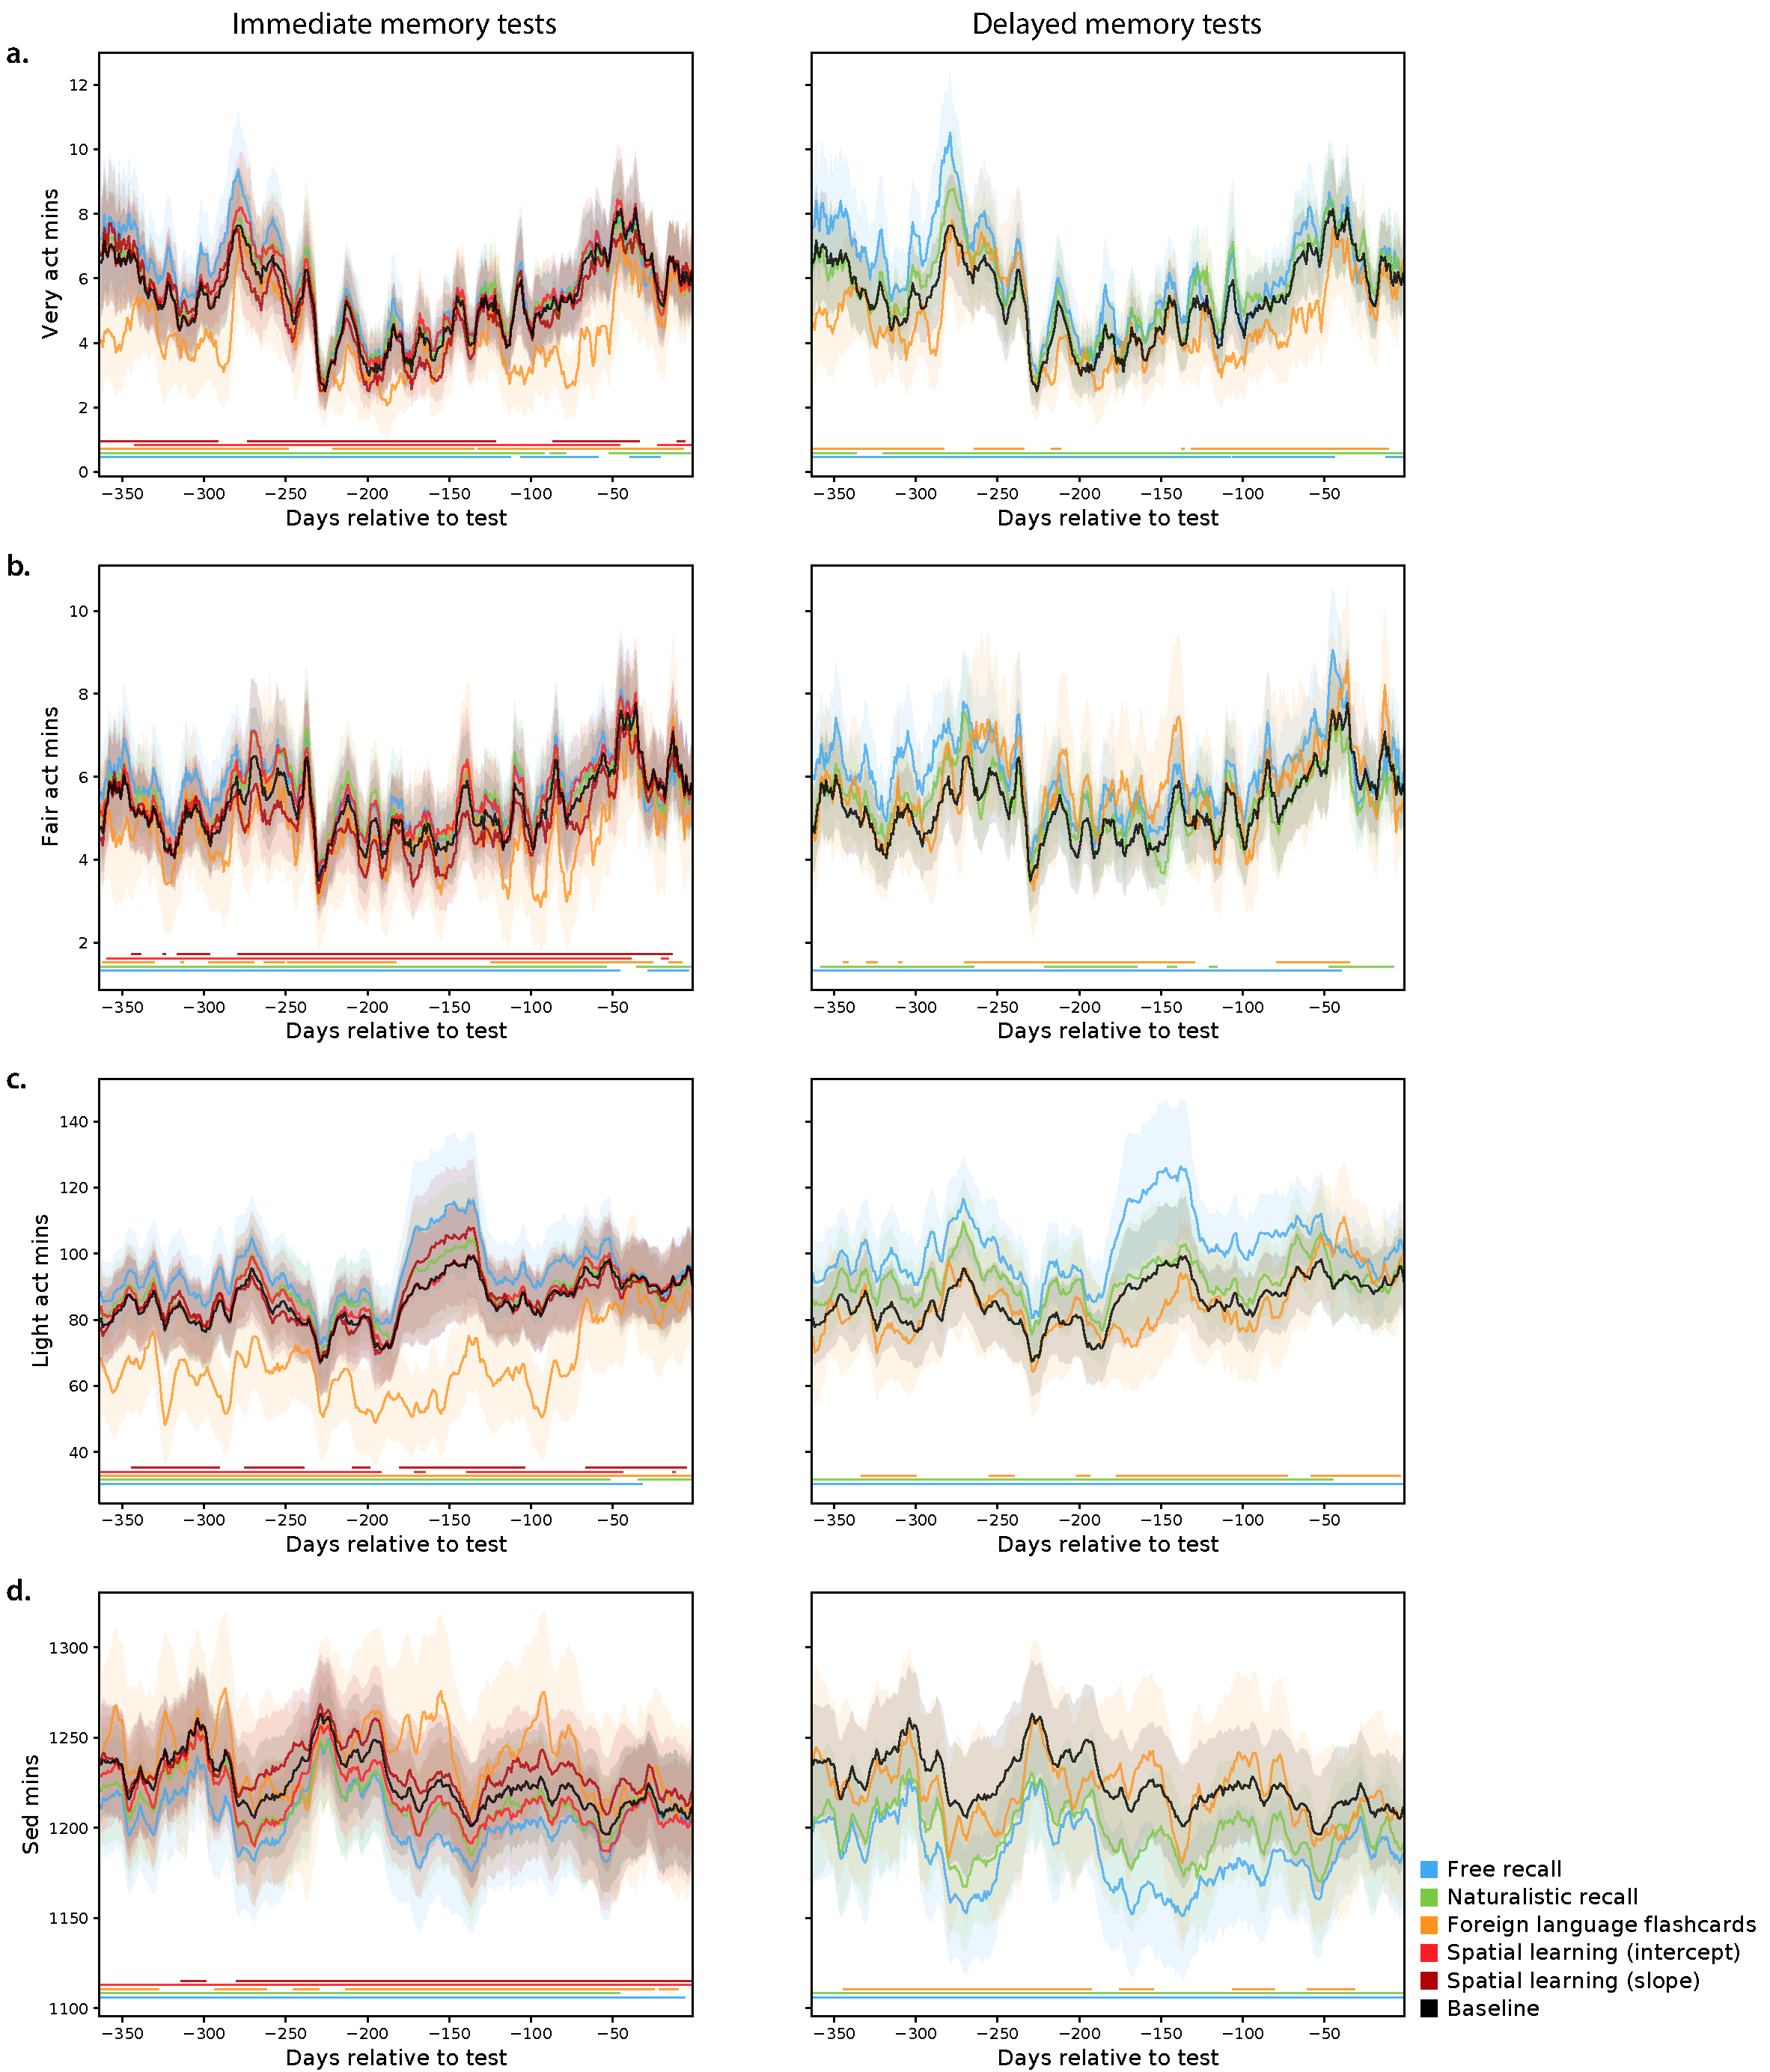
\includegraphics[width=0.75\textwidth]{figs/weighted_timecourse_activity}
\caption{\textbf{History of fitness activity levels weighted by
    behavioral performance.}  This figure is in the same format as
  Figure~\dynamics a and b, but shows additional fitness-related measures (Tab.~\ref{tab:abbreviations}).}
\label{fig:activity_timecourse}
\end{figure}

\begin{figure}[p]
  \centering
  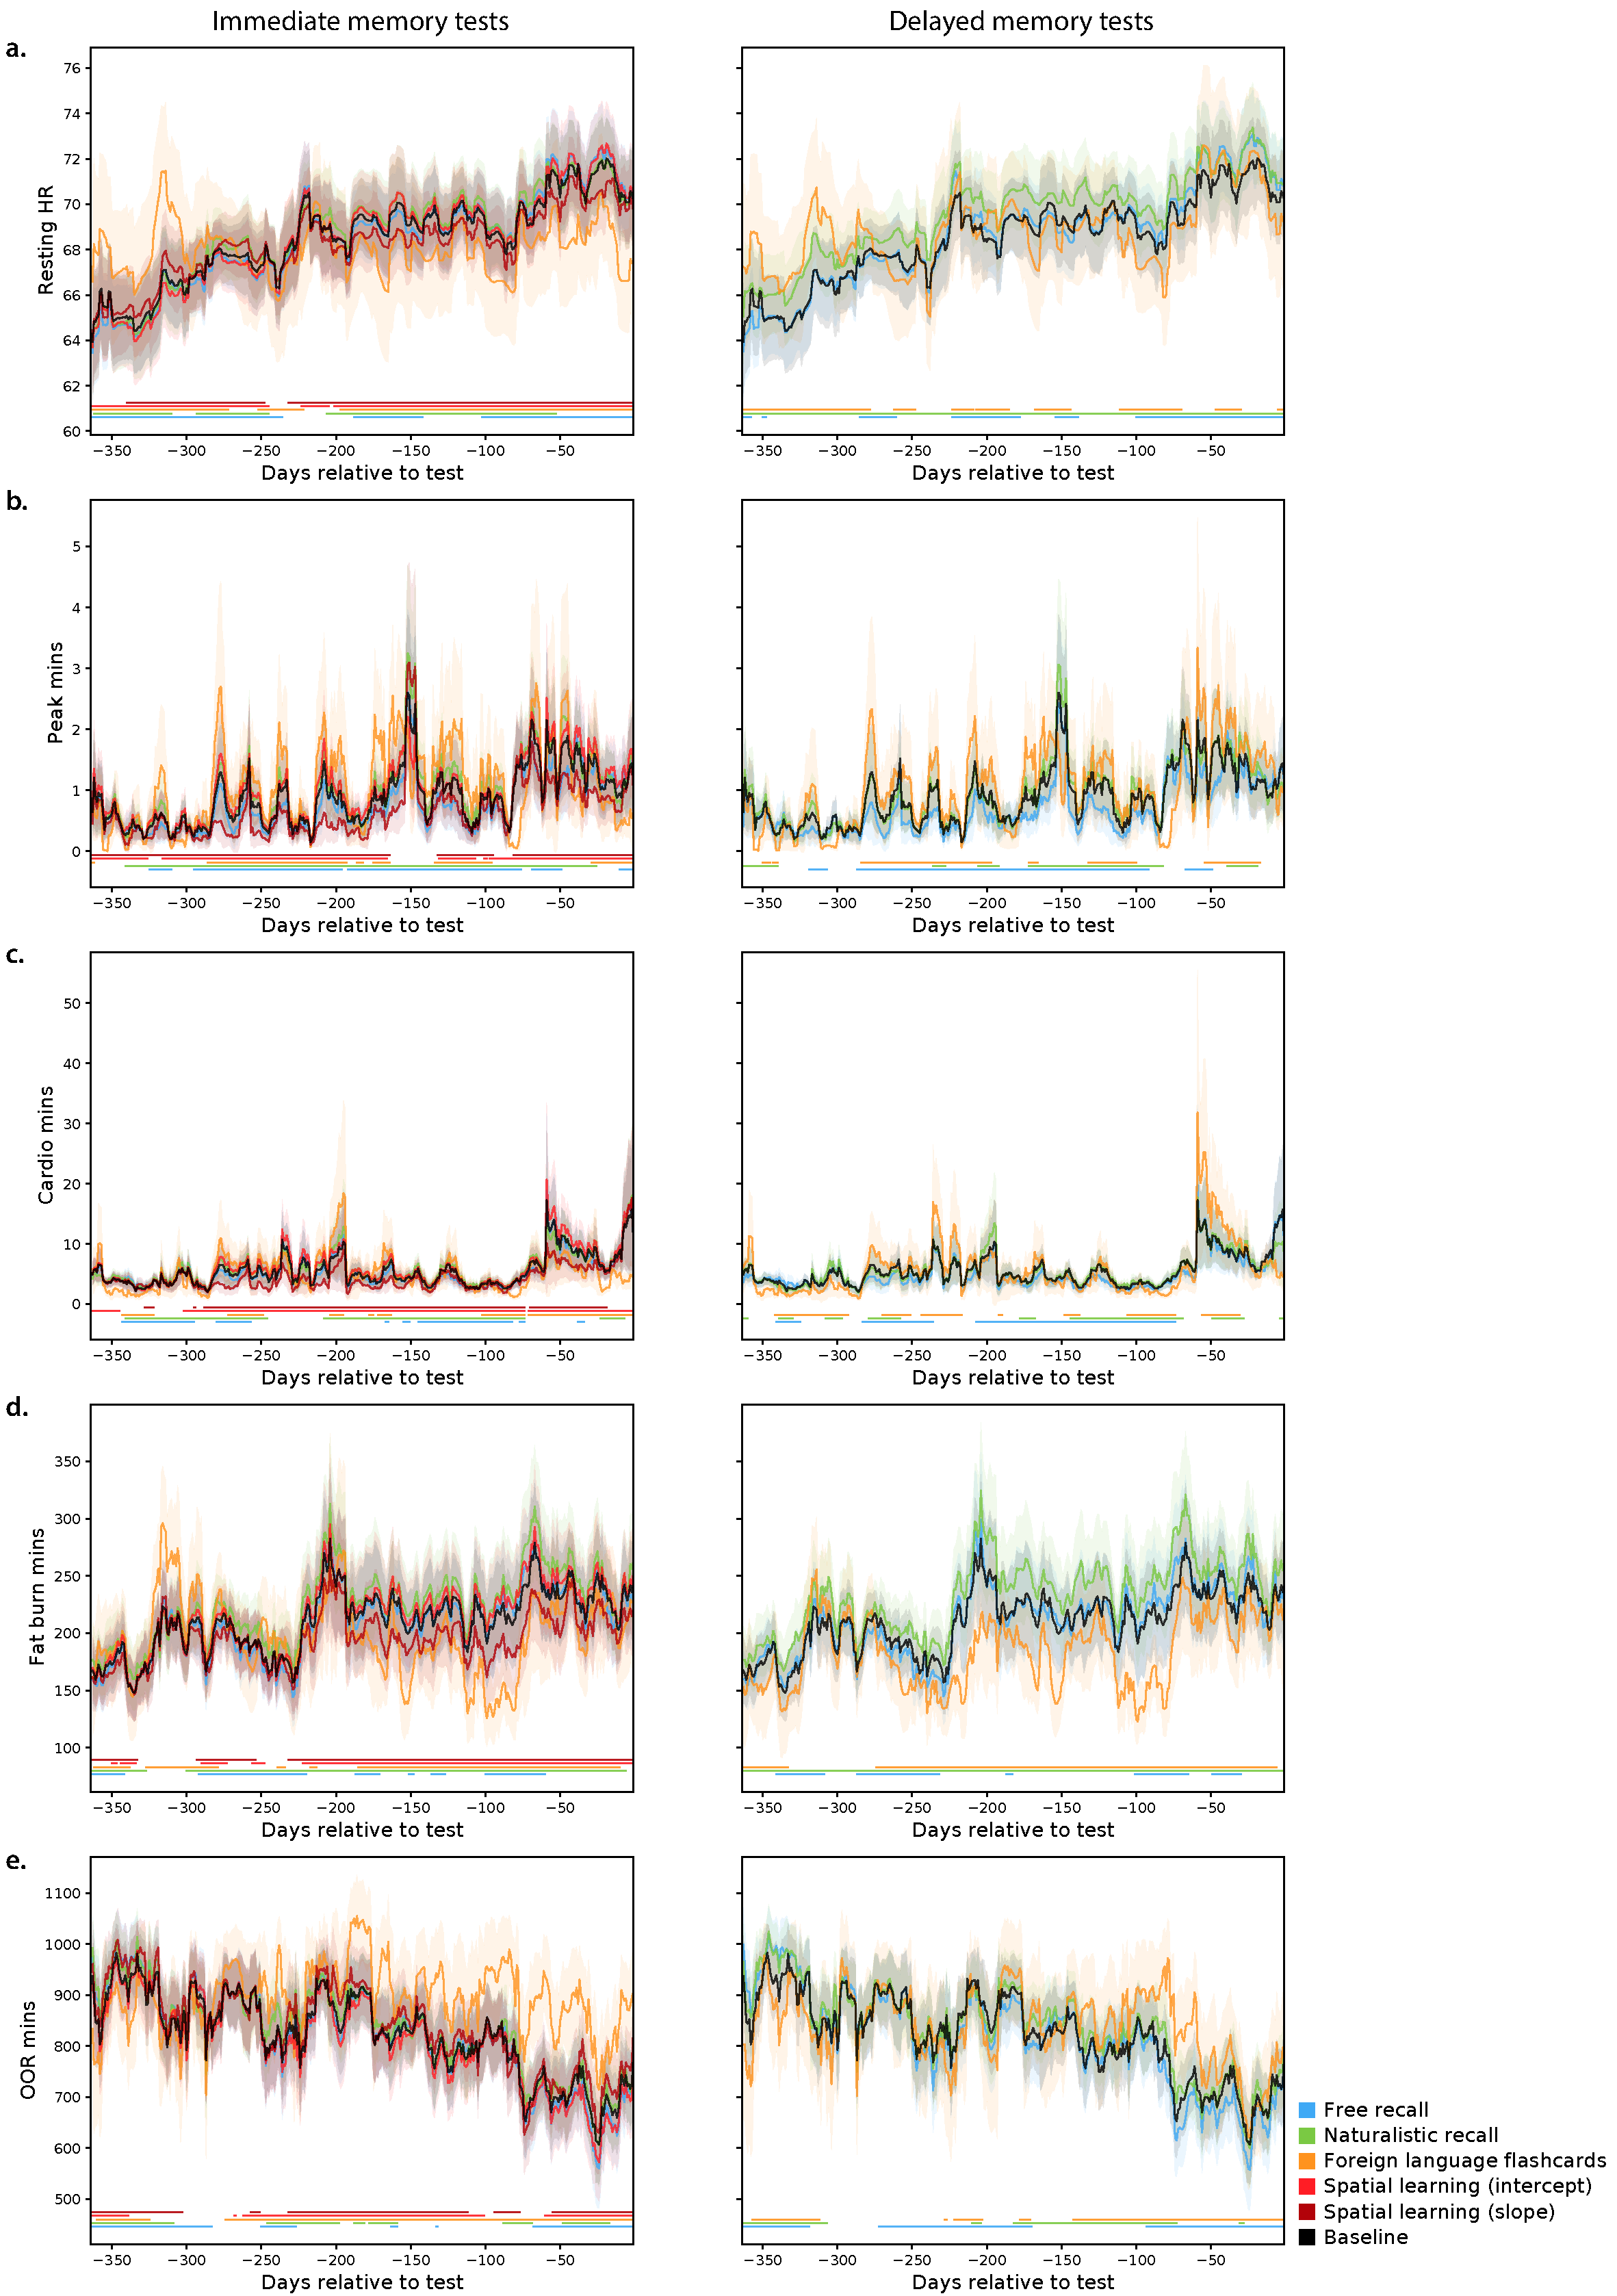
\includegraphics[width=0.7\textwidth]{figs/weighted_timecourse_HR}
\caption{\textbf{History of cardiovascular activity weighted by
    behavioral performance.}  This figure is in the same format as
  Figure~\dynamics a and b, but shows additional fitness-related measures (Tab.~\ref{tab:abbreviations}).}
\label{fig:HR_timecourse}
  \end{figure}

\begin{figure}[p]
  \centering
  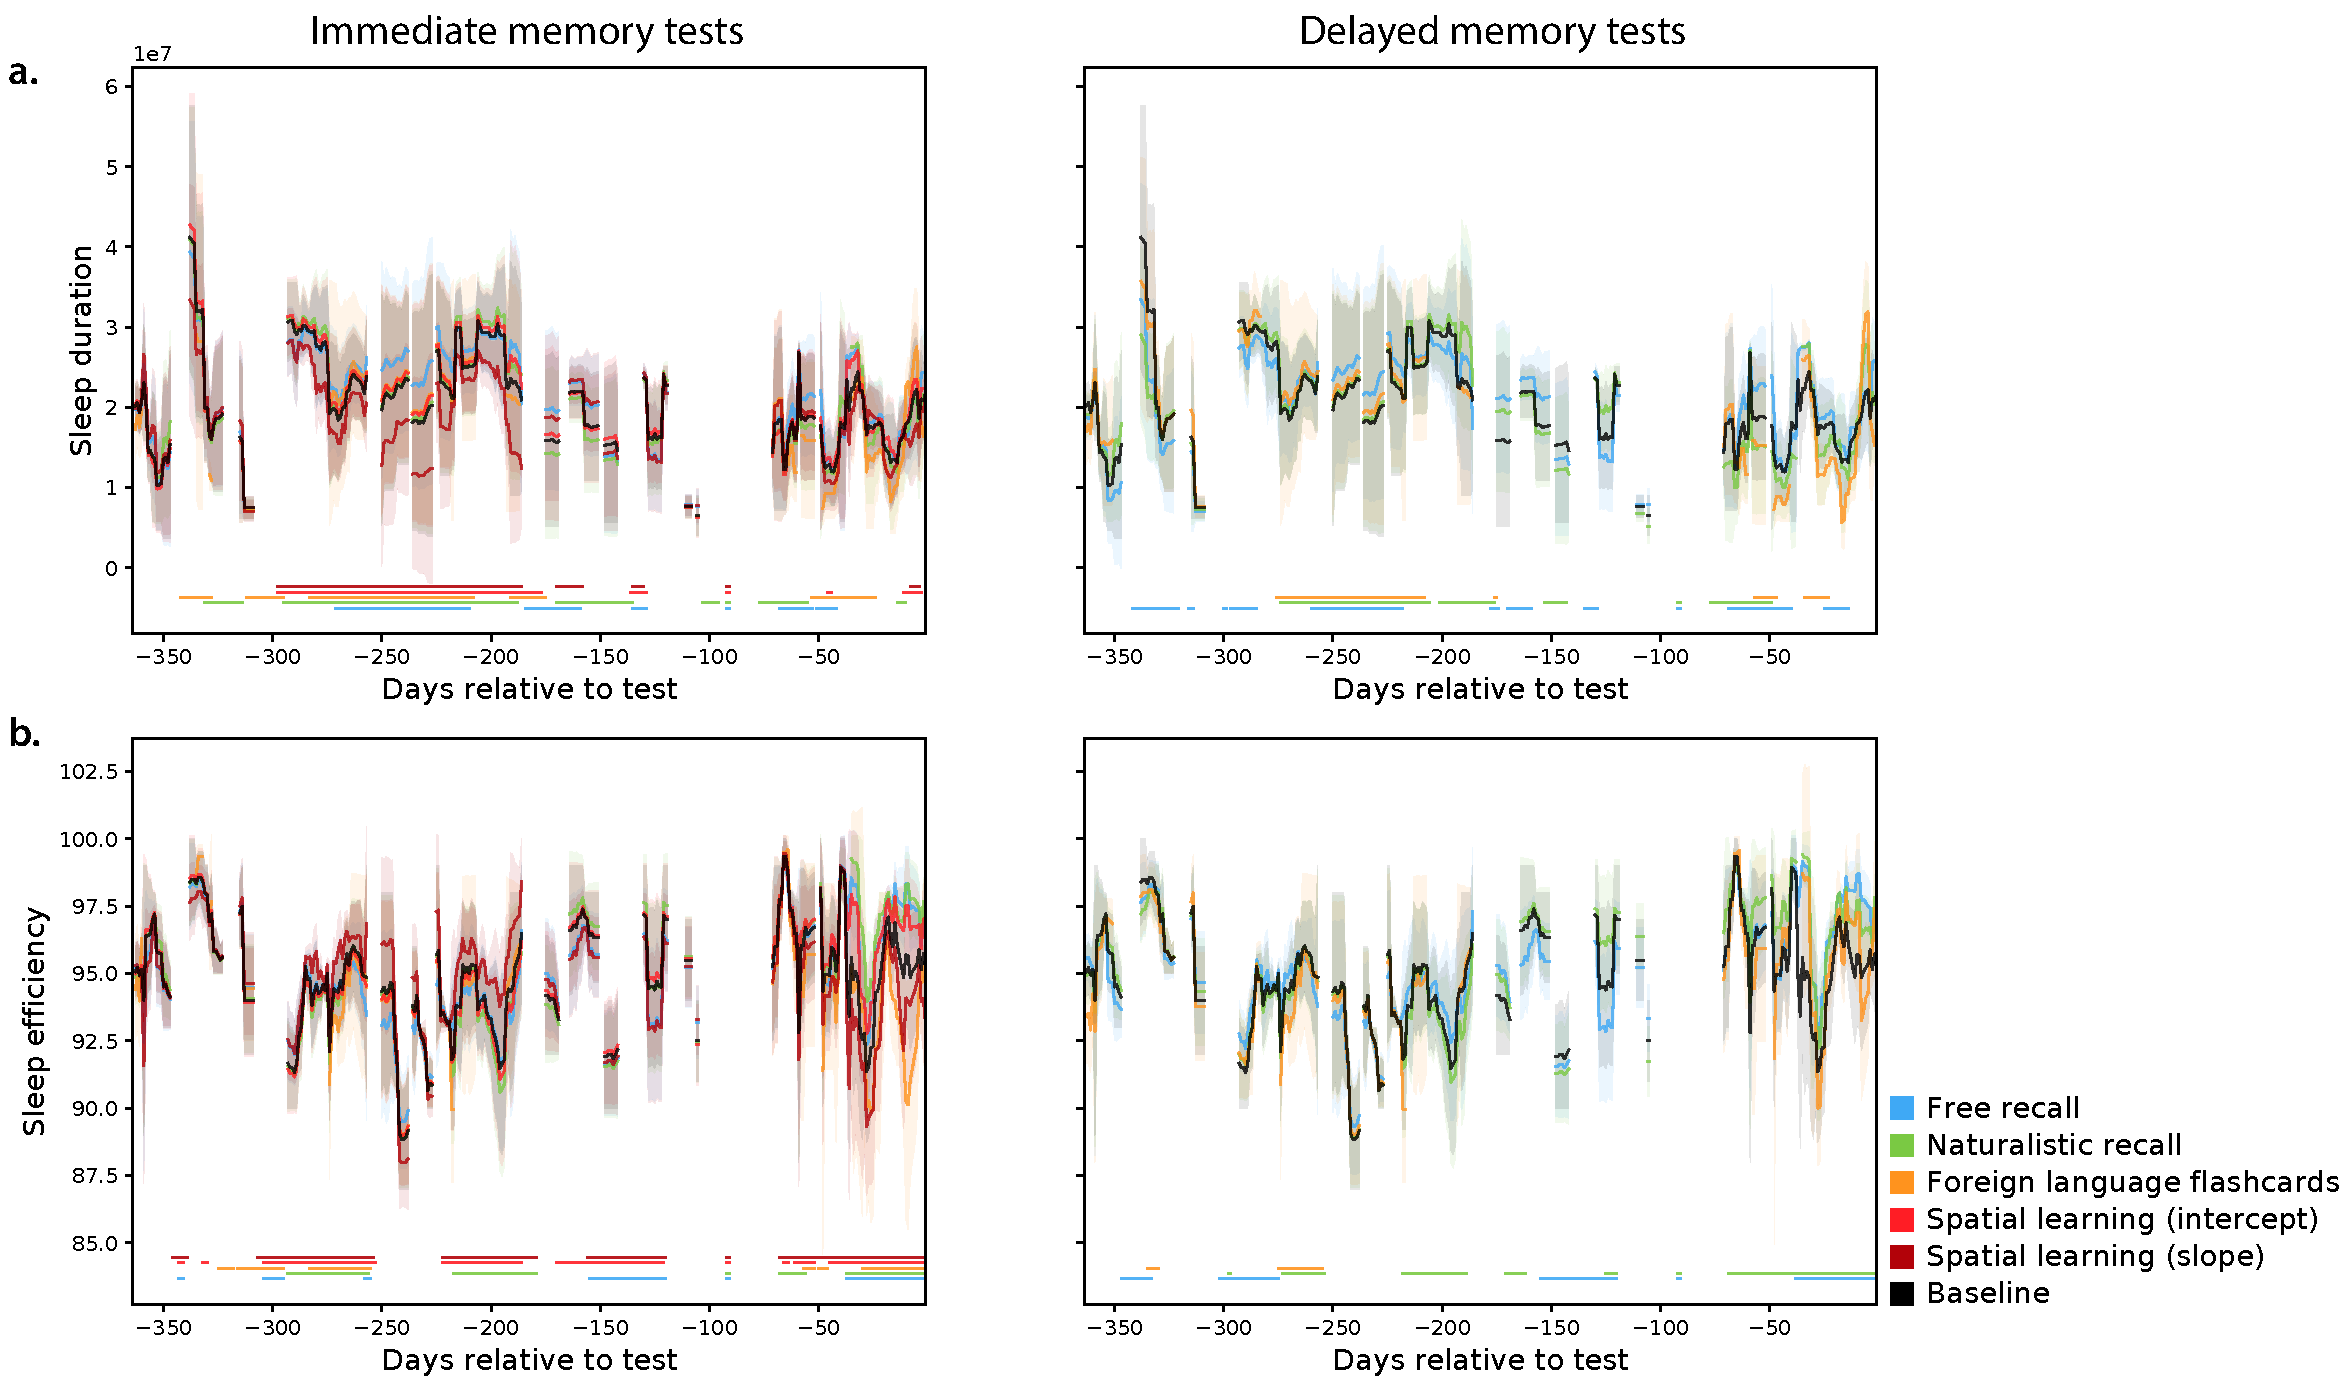
\includegraphics[width=0.75\textwidth]{figs/weighted_timecourse_sleep}
\caption{\textbf{History of sleep efficiency and duration weighted by
    behavioral performance.}  This figure is in the same format as
  Figure~\dynamics a and b, but shows additional fitness-related measures (Tab.~\ref{tab:abbreviations}).}
\label{fig:sleep_timecourse}
\end{figure}

\begin{sidewaysfigure}[p]
  \centering
  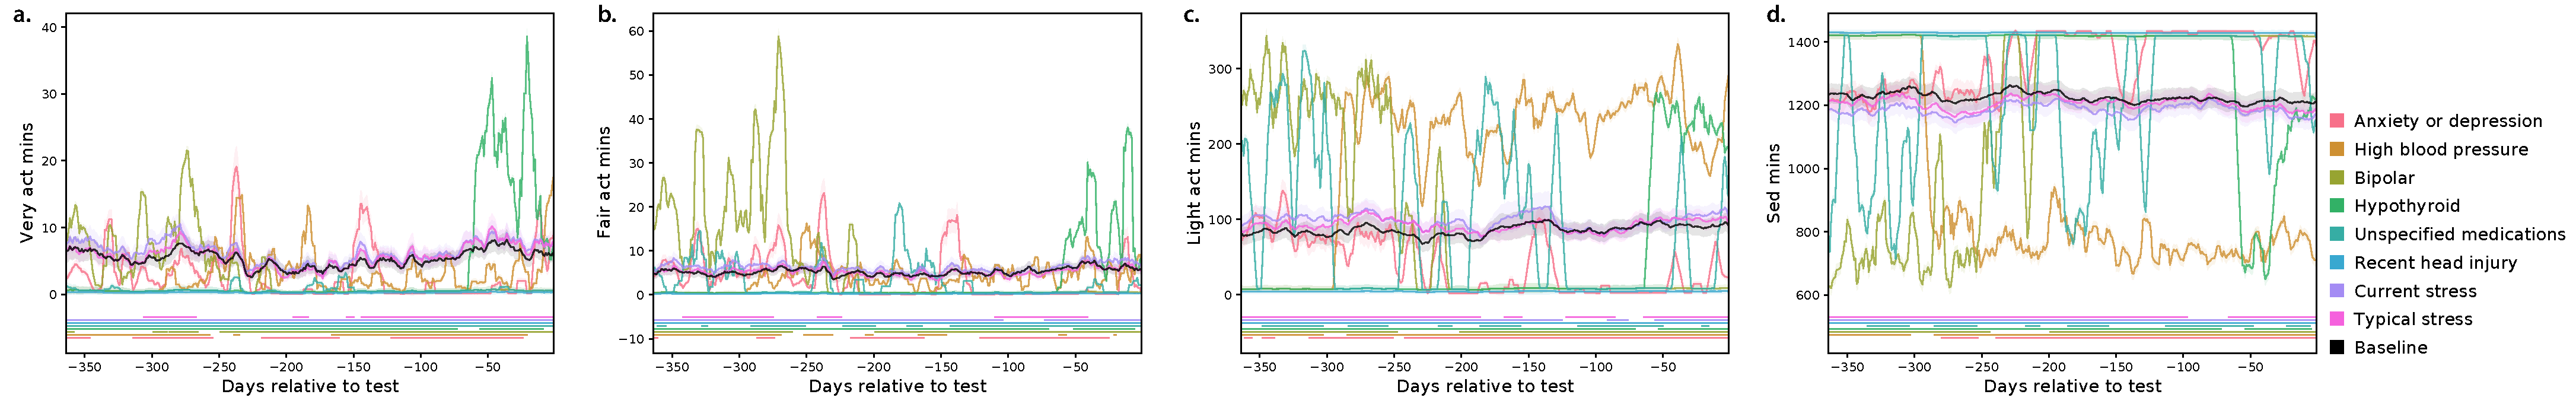
\includegraphics[width=0.75\textwidth]{figs/weighted_timecourse_activity_MH}
\caption{\textbf{History of fitness activity levels weighted by
    mental health factors.}  This figure is in the same format as
  Figure~\dynamics c, but shows additional fitness-related and mental
  health-related measures (Tab.~\ref{tab:abbreviations}).}
\label{fig:activity_timecourse_MH}
\end{sidewaysfigure}

\begin{sidewaysfigure}[p]
  \centering
  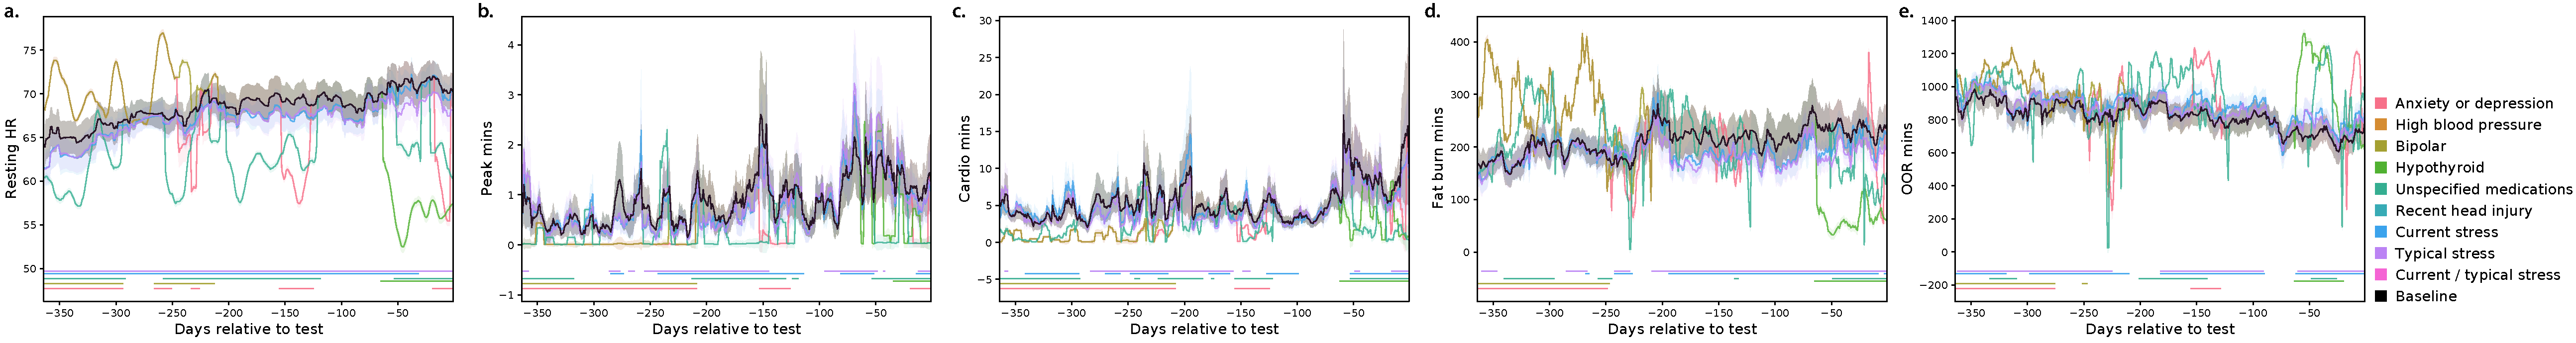
\includegraphics[width=\textwidth]{figs/weighted_timecourse_HR_MH}
\caption{\textbf{History of cardiovascular activity weighted by
    mental health factors.} This figure is in the same format as
  Figure~\dynamics c, but shows additional fitness-related and mental
  health-related measures (Tab.~\ref{tab:abbreviations}).}
\label{fig:HR_timecourse_MH}
  \end{sidewaysfigure}

\begin{figure}[p]
  \centering
  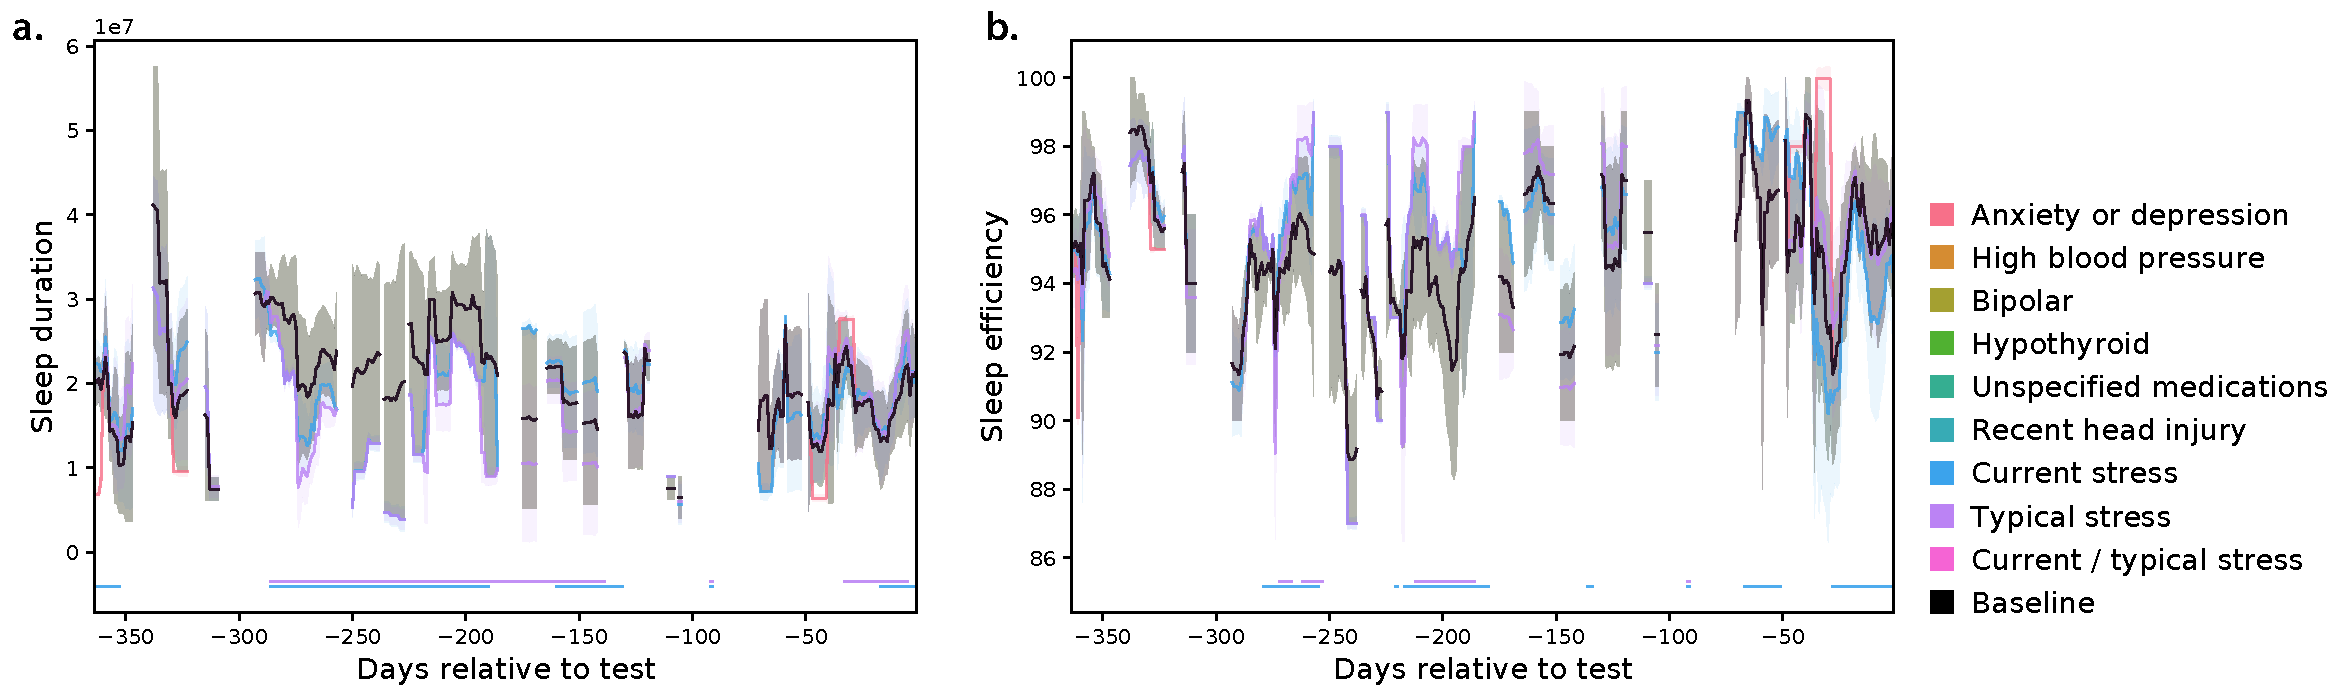
\includegraphics[width=0.75\textwidth]{figs/weighted_timecourse_sleep_MH}
\caption{\textbf{History of sleep efficiency and duration weighted by
    mental health factors.} This figure is in the same format as
  Figure~\dynamics c, but shows additional fitness-related and mental
  health-related measures (Tab.~\ref{tab:abbreviations}).}
\label{fig:sleep_timecourse_MH}
  \end{figure}

  \clearpage
  \newpage
\bibliographystyle{apa}
\bibliography{/Users/jmanning/CDL-bibliography/cdl}
\end{document}
